\documentclass{article} % Choose class of document

% Define required packages here 
\usepackage{nomencl}
\usepackage[margin=3cm]{geometry}
\usepackage[bottom]{footmisc}
\usepackage{setspace}
\usepackage{graphicx}
\usepackage{subcaption}
\usepackage{float}
\usepackage{import}
\usepackage{tabularx}

% Command for nomenclature which is defined here prior to the start of the document
\makenomenclature
\renewcommand{\nompreamble}{(The nomenclature must respect the following order: latin symbols, Greek symbols, acronyms. Within each category of symbols, follow alphabetic order. An example is provided below)}

% Set the spacing between lines of the document
\onehalfspacing

% The document commences here (everything above is used to set up the .tex file
\begin{document}

% Input the Title Page .tex file here (inputs have been used to collate the section and manage the document easier).
\begin{center}

    \begin{figure}[H]
        \centering
        
\includegraphics[width=7cm]{Images/UNSW Logo.png}
    \end{figure}

    \LARGE
    School of Mechanical and Manufacturing Engineering \\
    Faculty of Engineering \\
    UNSW Sydney

    \vspace{0.75cm}
    \LARGE
    BY \\
    \vspace{0.25cm}
    \huge
    \textbf{Chak Wang Choi} \\
    \vspace{0.5cm}

    \LARGE
    \textbf{Autonomous Visual Docking of a ROV onto a Moving Dock: Terminal Guidance in Simulation and Empirical Limits of ArUco Perception Underwater}
    \vspace{0.75cm}

    \LARGE
    Thesis submitted as a requirement for the degree of Bachelor of Engineering

    \vfill
    \large
    \begin{tabularx}{1\textwidth}{
            | >{\raggedright\arraybackslash}X
            | >{\raggedright\arraybackslash}X
            |}
        \hline
        Submitted: Aug 7th, 2026        & Student zID: z5413670 \\
        \hline
        Supervisor: Will Midgley (UNSW) &                       \\
        \hline
    \end{tabularx}
\end{center}


% Page breaks can be used to start a new page
\pagebreak

\input{Sections/Originality Statement}

\pagebreak

\section*{Abstract}
\addcontentsline{toc}{section}{Abstract}

This thesis focuses on the optical terminal stage of underwater docking using passive markers and computer vision, the approach available to low-cost ROV platforms that cannot carry learning-based perception. In simulation, a position-based visual servoing pipeline docks a BlueROV2 autonomously onto a swaying dock through two phases: coarse approach and fine alignment. In parallel, the operating envelope of passive ArUco perception is measured from real underwater imagery through analysis of detection range, pose error, and degradation with distance and turbidity. Together, these bound the operating range of marker-based terminal docking and identify where a paired complementary far-field cue becomes necessary.


\pagebreak

\section*{Acknowledgments}
\addcontentsline{toc}{section}{Acknowledgments}

% Acknowledge supervision and assistance.

I would like to thank my supervisor, Will Midgley, for guidance and support throughout the project. Also, thanks to Harrison Burns for helping with getting the simulation environment setup; thanks to Kushagra Javeri for access to the BlueROV2 and ZED camera, for the underwater camera work which part of this thesis builds on, and for assistance during pool testing; and to Jean-Henri Odendaal for fabrication and printing support for the waterproofed aruco markers.

\pagebreak

\tableofcontents

\pagebreak

\cleardoublepage

\addcontentsline{toc}{section}{List of Figures}
\listoffigures

\pagebreak

\cleardoublepage

\addcontentsline{toc}{section}{List of Tables}
\listoftables

\pagebreak

\addcontentsline{toc}{section}{Nomenclature}

% Order: Latin, Greek, acronyms; alphabetical within each. Edit/extend as needed.
% --- Latin ---
\nomenclature[1A]{\(A\)}{sinusoidal motion amplitude (m)}
\nomenclature[1B]{\(B_c\)}{backscatter / veiling-light colour (per channel)}
\nomenclature[1d]{\(d\)}{camera-to-marker range / scene distance (m)}
\nomenclature[1f]{\(f\)}{camera focal length (px)}
\nomenclature[1I]{\(I_c\)}{observed image intensity (per channel)}
\nomenclature[1J]{\(J_c\)}{clear-water (attenuation-free) radiance (per channel)}
\nomenclature[1r]{\(r\)}{relative range to dock (m)}
\nomenclature[1s]{\(s\)}{marker black-square side length (m)}
\nomenclature[1T]{\(T\)}{oscillation period (s)}
\nomenclature[1v]{\(v\)}{relative velocity (m/s)}
% --- Greek ---
\nomenclature[2beta]{\(\beta_c\)}{attenuation coefficient, per channel (1/m)}
\nomenclature[2sigma]{\(\sigma_{pos},\sigma_{rot}\)}{pose-estimate standard deviation}
\nomenclature[2tau]{\(\tau\)}{minimum inter-marker Hamming distance}
\nomenclature[2omega]{\(\omega\)}{angular frequency, \(2\pi/T\) (rad/s)}
% --- Acronyms ---
\nomenclature[3ArUco]{ArUco}{Augmented Reality University of Cordoba fiducial marker}
\nomenclature[3AUV]{AUV}{Autonomous Underwater Vehicle}
\nomenclature[3CV]{CV}{Computer Vision}
\nomenclature[3DOF]{DOF}{Degree(s) of Freedom}
\nomenclature[3EKF]{(M)EKF}{(Multiplicative) Extended Kalman Filter}
\nomenclature[3FNU]{FNU}{Formazin Nephelometric Unit (turbidity)}
\nomenclature[3FOV]{FOV}{Field of View}
\nomenclature[3IBVS]{IBVS}{Image-Based Visual Servoing}
\nomenclature[3IFM]{IFM}{(underwater) Image Formation Model}
\nomenclature[3PBVS]{PBVS}{Position-Based Visual Servoing}
\nomenclature[3PnP]{PnP}{Perspective-n-Point}
\nomenclature[3ROS]{ROS}{Robot Operating System}
\nomenclature[3ROV]{ROV}{Remotely Operated Vehicle}
\nomenclature[3SITL]{SITL}{Software In The Loop}
\nomenclature[3ZED]{ZED}{Stereolabs ZED stereo camera}

\printnomenclature


\pagebreak

\section{Introduction}
\label{sec:introduction}

Docking provides an underwater vehicle a place to recharge, offload its data and perform long-running tasks without surfacing or returning to a support ship. Since surfacing and recovery are slow, and weather-limited and expensive, removing them from the mission cycle is what makes long deployments and resident vehicle systems possible. The engineering challenge concentrates in the last few metres of the dock approach (Figure~\ref{fig:docking-problem}), in which if this stage goes wrong, the vehicle may collide with the dock, or abort and spend unnecessary time and energy retrying.

\begin{figure}[H]
    \centering
    % Annotated docking-problem figure for the Introduction.
% Image: Gazebo screenshot, BlueROV2 seen from behind on approach with the
% marker-equipped dock ahead. Coordinates are normalised to the image
% (0,0 = bottom left).
\begin{tikzpicture}
  \node[anchor=south west, inner sep=0] (img) {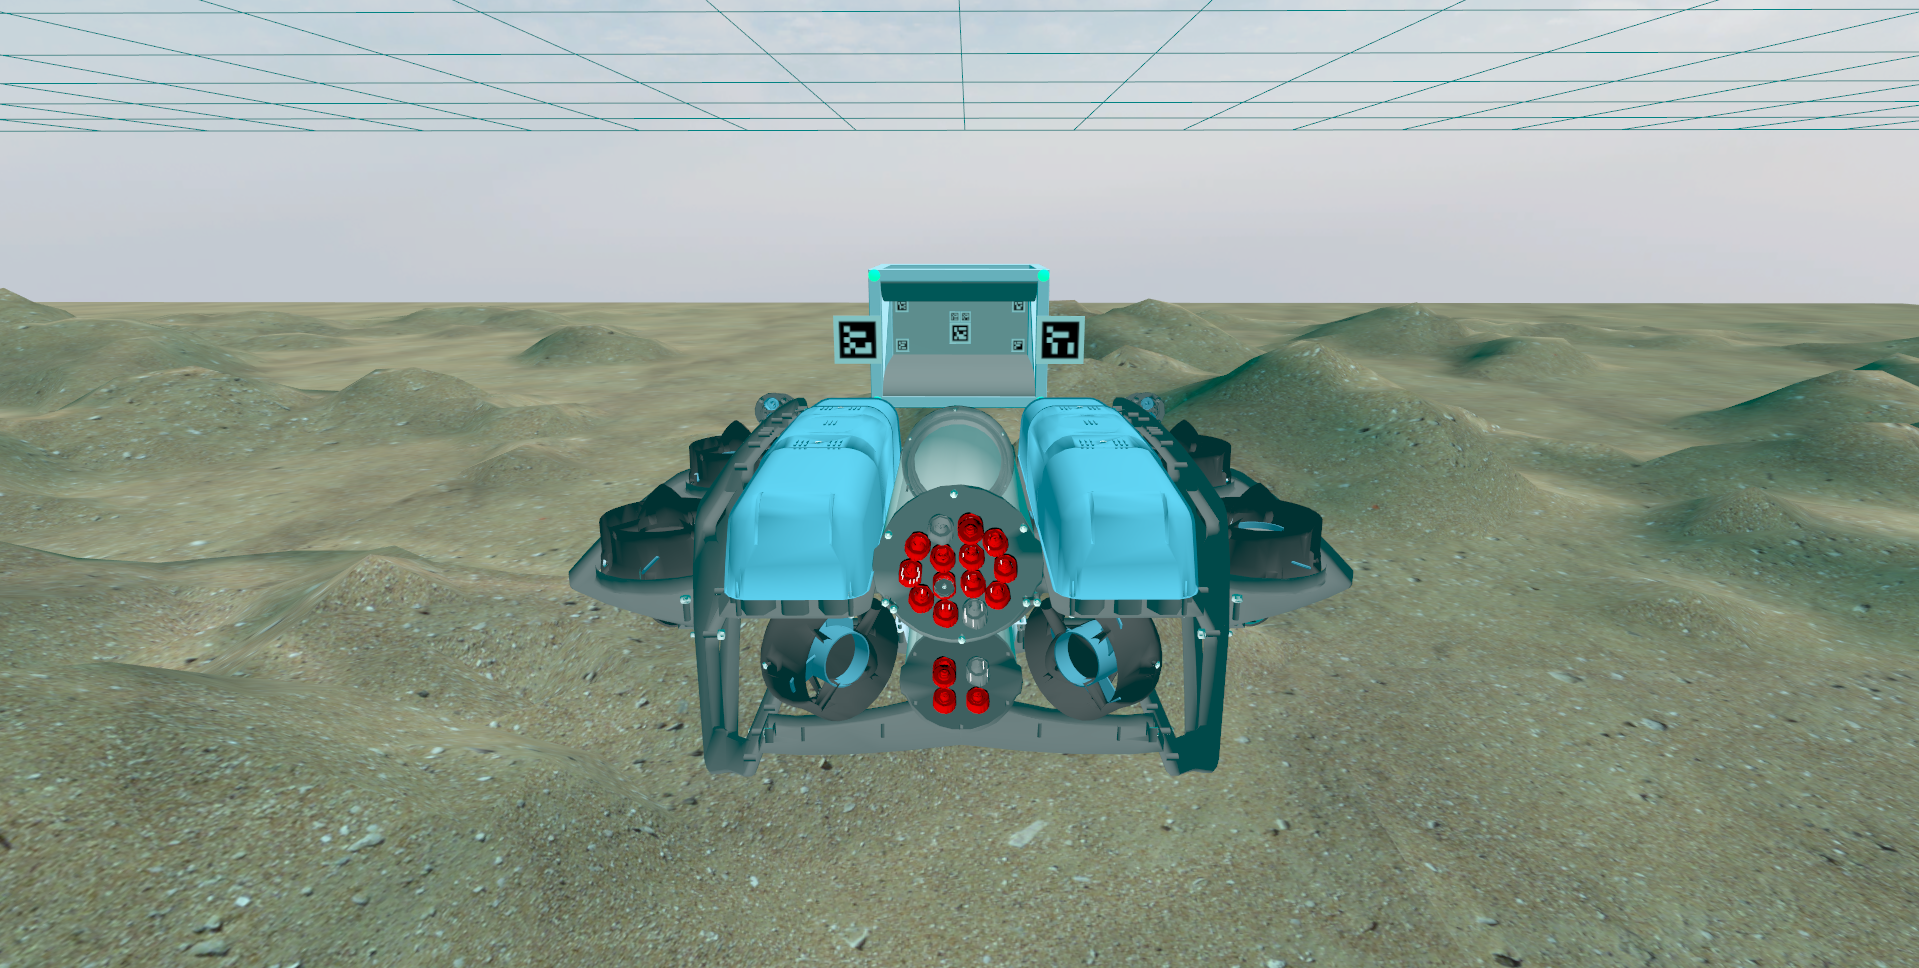
\includegraphics[width=0.85\textwidth]{Images/docking_problem.png}};
  \begin{scope}[x={(img.south east)}, y={(img.north west)},
    lab/.style={font=\scriptsize\bfseries, text=white, align=center, fill=black, fill opacity=0.55,
        text opacity=1, inner sep=3pt, rounded corners=1pt},
    arr/.style={orange, thick, -{Stealth[length=1.6mm]}}]
    \draw[white, thin, dashed, opacity=0.8] (0.50,0.56) -- (0.435,0.635);
    \draw[white, thin, dashed, opacity=0.8] (0.50,0.56) -- (0.565,0.635);
    \node[lab] (lrov) at (0.16,0.55) {BlueROV2\\forward camera};
    \draw[arr] (lrov.east) to[bend right=10] (0.36,0.44);
    \node[lab] (ldock) at (0.83,0.82) {docking station\\passive ArUco markers};
    \draw[arr] (ldock.south) to[bend left=10] (0.575,0.70);
    \node[lab] (lsway) at (0.24,0.82) {wave-driven sway};
    \draw[arr, <->] (0.41,0.77) -- (0.57,0.77);
  \end{scope}
\end{tikzpicture}

    \caption{The terminal docking problem: the vehicle must fly the final
        metres onto a docking station using its forward camera and marker detection, while the dock itself sways with the sea above.}
    \label{fig:docking-problem}
\end{figure}

Conventionally, a docking mission is staged by sensing modality, like acoustic or electromagnetic homing, to bring the vehicle from long range into the vicinity of the dock, then vision takes over for the final metres, where the precision requirement is tightest. This thesis addresses only the vision stage; homing and the mechanical capture are out of scope. Within the vision stage, two practical difficulties receive little attention in the literature. First, a real dock is rarely still, since moored and suspended structures inherit the wave motion of the sea around them. Second, the water limits how far a camera can see the dock at all, so marker visibility itself becomes a design constraint.

The work is split into two parts (Figure~\ref{fig:workflow}). Part~A develops the complete docking pipeline in simulation (marker fusion, a Kalman filter for the dock pose, and phase control) and runs it against a dock swaying at certain wave periods.\footnote{The docking stack and simulation fork are available at \url{https://github.com/alanchoi00/bluerov2-docking} and \url{https://github.com/alanchoi00/blue-sim}.} A docking trial sweep through the sway periods is performed to determine where the docking breaks down and the failure analysis explains why. Part~B takes the marker detector into real water where a pool capture measures detection against marker size, maximum detection range and the water's attenuation coefficient, and the same frames are then processed with artificial turbidity to produce a marker sizing rule. This split is necessary since the Gazebo simulator is able to exercise the closed loop, but cannot render water optics; the pool test captures have real optics but no control loop.

\begin{figure}[H]
    \centering
    \begin{tikzpicture}[font=\scriptsize, >={Stealth[length=2mm]},
  blk/.style={draw, rounded corners=2pt, align=center, inner sep=3pt, minimum height=6.5mm, minimum width=34mm},
  sumbox/.style={draw, rounded corners=2pt, align=center, inner sep=3pt, minimum height=6.5mm, minimum width=34mm, fill=black!6},
  lbl/.style={font=\scriptsize\bfseries, anchor=west}]

  % Part A column (closed-loop simulation)
  \node[blk] (a1) {swaying dock\\ \tiny Gazebo, wave-band periods};
  \node[blk, below=4.5mm of a1] (a2) {onboard camera};
  \node[blk, below=4.5mm of a2] (a3) {perception\\ \tiny marker fusion + Kalman filter};
  \node[blk, below=4.5mm of a3] (a4) {guidance and control\\ \tiny PBVS, coarse-to-fine state machine};
  \node[blk, below=4.5mm of a4] (a5) {vehicle motion};
  \draw[->] (a1) -- (a2);
  \draw[->] (a2) -- (a3);
  \draw[->] (a3) -- (a4);
  \draw[->] (a4) -- (a5);
  \draw[->] (a5.west) to[bend left=40] node[left, align=center]{\tiny moving\\ \tiny camera} (a2.west);

  % Part B column (real-water sensing, open loop)
  \node[blk, right=24mm of a1] (b1) {marker board in pool water\\ \tiny hand-held walk-backs};
  \node[blk, below=4.5mm of b1] (b2) {ArUco detection\\ \tiny scored per marker and frame};
  \node[blk, below=4.5mm of b2] (b3) {envelope measurements\\ \tiny detection vs apparent size, max\\ \tiny range, attenuation coefficient};
  \node[blk, below=4.5mm of b3] (b4) {synthetic turbidity stress\\ \tiny re-attenuate the same frames};
  \draw[->] (b1) -- (b2);
  \draw[->] (b2) -- (b3);
  \draw[->] (b3) -- (b4);

  % group boxes
  \node[draw, dashed, rounded corners=3pt, inner sep=3mm, fit=(a1)(a5)] (boxA) {};
  \node[draw, dashed, rounded corners=3pt, inner sep=3mm, fit=(b1)(b4)] (boxB) {};
  \node[lbl, anchor=south west] at (boxA.north west) {A: docking dynamics (sim)};
  \node[lbl, anchor=south west] at (boxB.north west) {B: sensing envelope (real water)};

  % synthesis
  \node[sumbox, below=8mm of $(boxA.south)!0.5!(boxB.south)$, minimum width=62mm]
  (syn) {operating envelope and dock design rules\\ \tiny sway-period limit, capture-interface numbers, pixel budget, marker sizing};
  \draw[->] (boxA.south) -- (syn.north -| boxA.south);
  \draw[->] (boxB.south) -- (syn.north -| boxB.south);
\end{tikzpicture}

    \caption{How the two parts fit together. The return arrow in Part~A is
        the closed control loop; Part~B is an open-loop measurement chain;
        their outputs combine into the envelope and design rules.}
    \label{fig:workflow}
\end{figure}

The objective of this thesis is to build and validate a terminal docking stage from passive markers and computer vision, the approach available to a low-cost ROV, and to establish its operating envelope. In simulation, the system docks autonomously onto a swaying dock, cleanly down to 8~s sway periods at 0.1~m amplitude. The swept periods are mapped to the NSW sea states to determine suitable dock depths. The sweep also uncovered a control instability: estimating the dock's velocity through a moving camera lets the vehicle's own motion corrupt the estimate, and at short sway periods this feedback destabilises the approach, while a simpler design that never estimates dock velocity is unaffected. On the sensing side, measurements on real underwater imagery established the perception envelope: a marker needs around 27 pixels of apparent size to be detected, maximum detection range is about 35 times the marker side, the water's attenuation coefficient was measured from the imagery itself, and inverting these numbers yields a sizing rule for the dock's markers.

Section~\ref{sec:literature-review} reviews the docking literature and states the research gap. Section~\ref{sec:methodology} describes the system and the experimental method for both parts. Section~\ref{sec:results} presents and discusses the results, and Section~\ref{sec:conclusion} concludes with future work.


\section{Literature Review}
\label{sec:literature-review}

% Target ~12-15 pages (be concise; significant info, not all info). Thematic, not
% chronological. End by making the research gap explicit -> sets up your contribution.

\subsection{Underwater docking: motivation and phases}

Autonomous Underwater Vehicle (AUV) docking has been a focus of research for decades, driven by the need for long-duration missions via subsea battery recharging and data transfer. A wide range of docking guidance strategies has been explored, as summarized in recent surveys \cite{yazdani2020survey}. Broadly, approaches are categorised by the sensing and guidance modality. Acoustic homing using sonar beacons can guide AUVs from long range, often providing range and bearing to a dock \cite{maire2009vision}. Electromagnetic docking systems have also been tested (e.g. using low-frequency EM fields for short-range homing), notably in Feezor's EM homing system \cite{feezor2001autonomous}. Vision-based techniques, using cameras to detect visual markers, offer high precision in final alignment. In practice, multi-modal solutions are common, where for example an AUV might navigate toward a dock via acoustic homing signals and then switch to vision-based guidance in the final meters \cite{maire2009vision}. Dedicated docking markers can be active (such as flashing lights or LED beacons) to increase visibility, or passive high-contrast patterns that require no power, as demonstrated in Maire's pole design. On the mechanical side, most docking station designs incorporate funnel-shaped guide surfaces to help capture the vehicle despite some misalignment. This combination of sensor guidance and mechanical alignment ensures a robust docking process under various conditions.

Numerous projects have demonstrated AUV docking with different infrastructures and homing strategies. One of the earliest was the WHOI REMUS AUV docking system from the late 1990s, which used a Relative Acoustic Tracking system of acoustic transponders for homing into a funnel-like subsea dock (see Figure~\ref{fig:remus-auv}) \cite{stokey1997docking, 4099107}.

\begin{figure}[H]
    \centering
    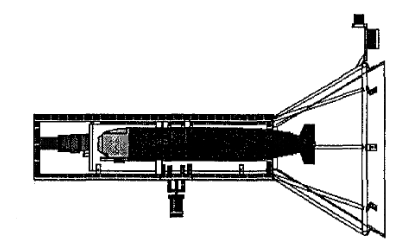
\includegraphics[width=0.6\textwidth]{Figures/remus-auv.png}
    \caption{A side-view drawing of the WHOI REMUS AUV docking system \cite{stokey1997docking}.}
    \label{fig:remus-auv}
\end{figure}

\noindent Researchers have since tested seabed-mounted and moored docking stations to support AUV missions. For instance, Maire et al. (2009) proposed a heavy weighted docking target pole lowered to the seafloor, equipped with an acoustic beacon for long-range localisation and a visual pattern for final approach. An AUV can home to such a seafloor station, attach itself, and enter a sleep or recharge mode until the next mission window \cite{maire2009vision}.

\begin{figure}[H]
    \centering
    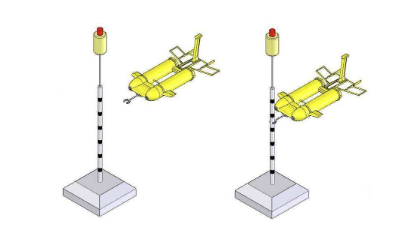
\includegraphics[width=0.6\textwidth]{Figures/maire-dock-diagram.png}
    \caption{Maire et al.'s seabed docking station concept with acoustic and visual homing aids. (left: on approach, right: after docking) \cite{maire2009vision}}
    \label{fig:maire-dock}
\end{figure}

\noindent Remotely operated vehicles (ROVs), being tethered and human piloted, traditionally dock via their tether management system (TMS), a cage lowered from the surface into which a pilot must manually fly the vehicle. Trslic et al.\ demonstrated the first autonomous TMS docking of a heavy work-class ROV in open ocean conditions, using vision-based pose estimation of the four active light markers on a conventional TMS cage (Figure~\ref{fig:trslic-cage}). The trials demonstrated repeated autonomous dockings to the suspended, heaving cage in January North Atlantic sea conditions \cite{trslic2020vision}.

\begin{figure}[H]
    \centering
    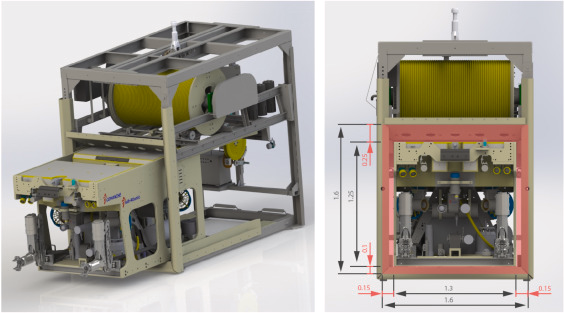
\includegraphics[width=0.6\textwidth]{Figures/trslic-dock-cage.png}
    \caption{The tether management system docking cage for work-class ROVs used in the first autonomous TMS docking demonstration \cite{trslic2020vision}.}
    \label{fig:trslic-cage}
\end{figure}

\noindent In a different configuration, researchers have also developed hybrid docking setups where an ROV acts as a mobile docking station to service AUVs. Morinaga et al.'s docking station ROV captures an AUV using electromagnets, and a slider device then aligns the receiving and transmitting antennas for inductive power transfer (see Figure~\ref{fig:morinaga-auv-flow}). The concept was demonstrated in a water tank docking test \cite{morinaga2021development}.

\begin{figure}[H]
    \centering
    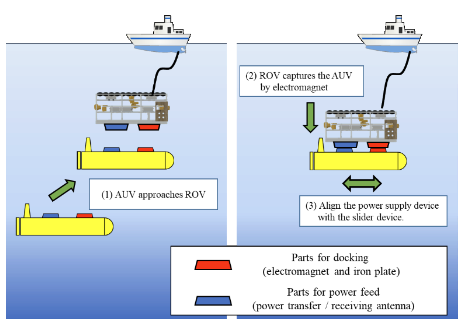
\includegraphics[width=0.6\textwidth]{Figures/morinaga-auv-flow.png}

    \caption{A flowchart of ROV-AUV docking interaction from Morinaga et al. \cite{morinaga2021development}}
    \label{fig:morinaga-auv-flow}
\end{figure}

This illustrates the breadth of ROV-involved docking solutions, from launch and recovery systems to ROVs serving as docking stations for AUV support. Across these systems, the common structure is a two-phase mission, in which long-range homing is followed by short-range terminal alignment. This thesis addresses the terminal phase.

\subsection{Acoustic and electromagnetic guidance}

Acoustic-based navigation is widely used as the long-range guidance channel for underwater docking. A common configuration has an acoustic transceiver on the dock that emits a signal, which is received by a transponder on the AUV. The AUV then replies with its own signal, allowing the dock to compute the distance based on the time delay. To obtain bearing information, several inverted ultra-short baseline (iUSBL) receivers are spaced precisely on the AUV hull. By measuring the slight time difference of arrival of the acoustic signals at each receiver, the system can triangulate the relative azimuth and elevation angles between DS and AUV. WHOI's REMUS AUV docking system is a prime example of a USBL-navigation aided system \cite{4099107}. Its acoustic homing can guide the AUV from long range, at the cost of moderate update rates, latency due to the speed of sound underwater, risk of false signals from acoustic refraction and ambient noise, and limited angular resolution.

Electromagnetic (EM) guidance offers an alternative to acoustic signals, using low-frequency magnetic fields emitted by a coil on the dock, and results in lower latency. Feezor et al. (2001) developed an EM homing system where a low-frequency magnetic field is generated by a coil on the dock, and the AUV uses magnetometers to detect the field strength and direction, without line-of-sight constraints \cite{feezor2001autonomous}. Their experiments demonstrated that the AUV could home in on the dock from a limited range up to $\sim$30~m. Further, the system requires dedicated coils, drivers and calibration of the local field environment, which may limit its practicality for general-purpose docking stations.

Most underwater docking stations incorporate mechanical alignment aids to relax the sensing requirement and accommodate for the slight tolerances during the final docking alignment phase. There exist two main configurations: unidirectional and omnidirectional guides. Unidirectional stations are the most common type of configuration, typically designed for a torpedo-shaped vehicle approaching on a known heading. Omnidirectional stations allow approach from any heading, typically as a vertical pole or tensioned cable, allowing the vehicle to be latched onto the dock despite its orientation, notably in the Odyssey IIb AUV's dock system \cite{972084}, simplifying the navigation and alignment process at the cost of a dedicated latch mechanism on the vehicle nose. In either configuration, the guide's capture radius and tolerated closing speed define the interface between the guidance problem and the mechanical one, in which the capture envelope assumed in this work (Section~\ref{sec:method-experiment}) plays that role.

\subsection{Dock motion in ROV operations}
\label{sec:lit-dock-motion}

During operational practice, the docking target is rarely still in place. For instance, Trslic's docking system has a work-class ROV recovered into a TMS cage suspended from its support vessel, and the cage inherits the vessel's wave-driven motion through the lift wire. Manual TMS docking requires the pilot's full concentration and skill, flying into a cage whose heave, yaw and pendulum swing follow the sea state, while decisions are taken in fractions of a second \cite{trslic2020vision}. The first autonomous TMS docking trials were run in dynamic North Atlantic wave conditions and were motivated by exactly this difficulty, with the objective to widen the operational weather window that the task currently dictates \cite{trslic2020vision}. In some concepts, the dock is not even a fixed structure. A docking-station ROV captures and recharges an AUV in the water column, so both the dock and the AUV are free bodies in the system \cite{morinaga2021development}. Even purpose-built resident docking stations are not still, since they are typically moored or suspended structures rather than rigid foundations. Dynamic analysis of a seabed-moored suspended dock shows it responds measurably to ocean-current forcing transmitted through its mooring line \cite{guo2024dynamic}.

This phenomenon of forcing on underwater object's motion is ordinary ocean physics. Ocean surface waves carry their energy at period of roughly 5 to 20~s (crest-to-crest times). Waves raised by the local wind sit at the short end of this band (5 to 8~s period), while swell arriving from distant storms has longer periods (above ~8~s) \cite{holthuijsen2007waves}. Below the surface, the wave orbital motion decays exponentially with depth at a rate set by the wavelength, while wavelength grows with the square of the period, so short wind sea is filtered out within tens of metres of depth while long-period swell induces wave motion far deeper \cite{holthuijsen2007waves}. A moored dock, therefore, oscillates with a period-dependent amplitude. In a typical sea, the motion surviving at continental-shelf depths is still of order 0.1~m, and because decay depends on period, a dock's depth determines which wave periods reach it. Off the NSW coast, the operating context of this work, the long-term mean sea state is a wave height of 1.6~m at a mean period of 8~s \cite{short1992wave,kinsela2024nearshore}, which places realistic dock motion within the wave band swept in Part~A. The quantitative mapping from period and depth to dock displacement is developed with the experimental design in Section~\ref{sec:method-sim}.

Against this operational picture, the docking control literature almost always models the dock as a fixed pose in the world frame, and where environmental disturbance appears, it is a steady current applied to the vehicle. The exceptions are partial. Trslic et al.\ docked to a heaving TMS cage by servoing on the most recent measured pose, reacting to the motion without having to model it \cite{trslic2020vision}. The same group later showed that TMS heave can be predicted (about 2.5~s ahead with a neuro-fuzzy model), but the prediction came from a pressure sensor mounted on the TMS cage itself, which only covers heave and was evaluated offline instead of in closed-loop docking \cite{trslic2020neuro}. Neither line of work estimates the dock's motion through the vehicle's own camera while both bodies are moving. The estimation problem that configuration raises is taken up in Section~\ref{sec:lit-estimation}.

\subsection{Vision-based docking and fiducial markers}

Passive visual markers are high-contrast patterns (typically black and white pixelated squared markers) detected by a camera and used for pose estimation. Early work from Maire's Starbug dock system designed custom geometries which used a binary encoded pole as a passive black and white target mounted inside a suspended docking station. The pattern is designed so that it is visible from any arbitrary yaw, roll or pitch angle and also serves as a structural station that the AUV can grip on. Detection is performed with a fast Haar feature template matcher over the image, where the 'dash-dot-dash' black and white pattern is scored over multiple scales, positions and image rotations to locate the camera pose relative to the dock \cite{maire2009vision}. As the AUV approaches closer, the system switches to shorter templates to maintain more precise tracking at close distance. This method purely using a high contrast pattern can deliver robust homing without any powered beacons, however, it is limited by the CPU cost of the template search over multiple scales and rotations, and restricts design flexibility for the dock station. Later work on general visual application for regular (standardised) fiducial systems like AprilTag and ArUco follows the standard method of obtaining pose of the markers from camera frame, which square markers are detected by adaptive thresholding and decoded against a dictionary, with the four corners feeding a Perspective-n-Point (PnP) solution for full 6-DOF pose \cite{garrido2014automatic, kalaitzakis2021fiducial}. Notably, Xu's AUV navigation system detects a grid of multiple markers for improved accuracy \cite{xu2021underwater}. The ArUco library first decodes each marker ID and recovers the marker's pose relative to the camera. Then, Xu's custom noise model computes an optimal combined pose estimate from all visible markers, improving accuracy and robustness against individual detection errors. Vision positioning with two cameras has likewise been used in AUV docking experiments \cite{li2015auv}. The same principle applies to Romero-Ram\'irez's fractal markers, which survive across the long to short range span by having ``an aggregation of squared markers, one into another, in a recursive manner'', see Figure~\ref{fig:fractal-marker} \cite{romeroramirez2019fractal}.

\begin{figure}[H]
    \centering
    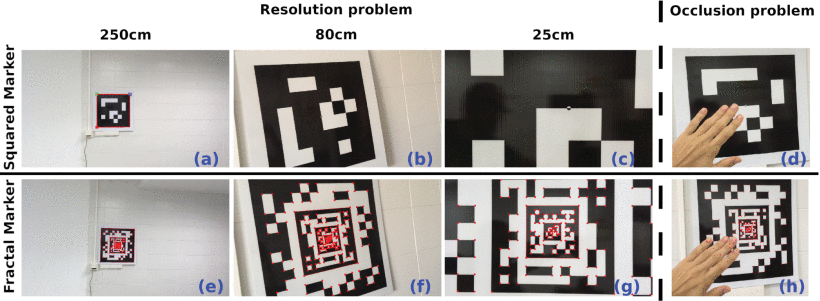
\includegraphics[width=0.6\textwidth]{Figures/fractal_markers_new_approach.png}
    \caption{Result of the Fractal Markers against regular squared markers at different distances and occlusion, where Fractal Markers can be detected in more cases than regular squared markers \cite{romeroramirez2019fractal}.}
    \label{fig:fractal-marker}
\end{figure}

\noindent There is little design guidance on how these marker sets should be arranged. Wang's controlled study on marker size, count and distribution found that apparent size is the dominant factor for localisation accuracy, while marker count and placement only have secondary effects \cite{wang2023effect}. The dock layout of this work assumes the same ordering. The closest deployed system to this work is G\"unzel's resident mini-ROV, which docks onto a multi-size ArUco layout at 90~m depth, fused through an extended Kalman filter, and reports a 90\% docking success rate \cite{gunzel2026docking}. This architecture matches the size-graded layout and filter design of this work. However, the dock station is static, and the marker sizes were selected through simulator experiments without water optics, so the underwater perception envelope remains unmeasured. For underwater detection performance, dos Santos Cesar et al. evaluated three fiducial systems (ArUco, AprilTag and ARToolKit) in tank conditions, measuring the smallest detectable size, maximum viewing angle and detection range across six turbidity levels \cite{cesar2015evaluation}. This study establishes apparent size and turbidity as the two main variables of underwater fiducial detection. Among the three libraries, ArUco showed the highest sensitivity to turbidity, with its required marker size growing at the fastest rate.

Most recently, Ni et al. proposed a hybrid active and passive docking marker where a printed AprilTag is placed at the center of the dock station, surrounded by an array of five LED lights \cite{ni2025vision}, following Trslic's four light beacon active marker design \cite{trslic2020vision}. A custom YOLO-D model is trained to simultaneously detect the LED array and the AprilTag in raw underwater images.
\begin{figure}[H]
    \centering
    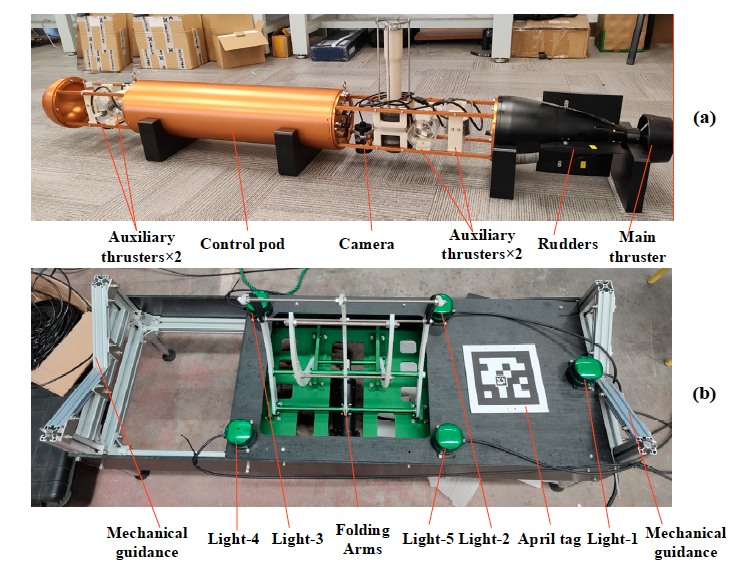
\includegraphics[width=0.6\textwidth]{Figures/msae-dock-and-auv-diagram.png}

    \caption{Example of an underwater docking station and vehicle: (a) AUV; (b) Docking station with five green LED beacons (Light-1 to Light-5), AprilTag marker at the center and v-shaped mechanical guides.\cite{ni2025vision}}
    \label{fig:ni-dock}
\end{figure}
\noindent Ni et al.'s AUV docking guidance is composed of two levels of detection:
\begin{itemize}
    \item Level I: the LED array is used as visual markers for pose estimation. However, at close range, the light scattering can introduce errors in estimating the center of the guidance light source.
    \item Level II: the AprilTag is used for precise pose estimation. However, this guidance method is limited by the detection range and visibility of the tag under turbidity, water quality and illumination.
\end{itemize}
The docking process begins by capturing an image, which is preprocessed through configured filters to minimise noise in the image. The YOLO-D model then detects the center \(X_L\) of the LED array and the AprilTag region of interest (ROI) in the image frame. In Level I guidance, the obtained \(X_L\) is used to compute a coarse position \(P_L\) of the docking station relative to the AUV. In Level II guidance, the AprilTag corners \(X_A\) are extracted from the ROI and used to compute a precise pose \(P_A\) via PnP. Finally, the pose estimates from both levels are fused to compute the overall \(P_{out}\), following the formula

\[ P_{out} = K_1 P_L + K_2 P_A \]

where \(K_1\) and \(K_2\) are weight matrices adjusted according to the conditions, shifting toward the surviving channel when poor water quality prevents one marker type from being detected. This fusion allows the system to leverage the long-range detection of the LED array while maintaining the precision of the AprilTag when visible.

Learning-based detection is the other active research direction. Standard object detectors are typically trained on terrestrial images, so their performance degrades in low-light and low-contrast conditions \cite{DAS20253042}, which are the typical conditions of underwater scenes, and motivated a few underwater-specific variants. For example, Pan's YOLOv9s-UI adds attention modules for underwater object detection \cite{app14167162}, and Ni's YOLO-D (described above) augments a YOLO backbone with multi-scale feature fusion and adaptive kernels to detect distant lights and partially visible tags \cite{ni2025vision}. Another, Sans-Muntadas trained a CNN that regresses the heading error to the dock directly from raw images, replacing explicit marker detection entirely \cite{sans2019learning}. However, this method degrades at close range where visible features vanish. In practice, these learning methods serve as the detection front end of a larger system, while the metric pose is still recovered geometrically from the marker corners. They also carry extra costs in training data, onboard compute and validation effort, which are significant for small / low-cost ROV platforms. For this reason, this thesis stays with the classical fiducial pipeline. The detection algorithm is mature and cheap, and the open question is the operating envelope of the detector rather than the detector itself.

\subsection{Visual servoing and guidance for docking}

Visual servo control divides into two schemes. Image-based visual servoing (IBVS) regulates the feature error directly in the image plane, while position-based visual servoing (PBVS) reconstructs a metric relative pose and regulates it in Cartesian space \cite{chaumette2006visual}. In this work, the perception layer already produces a full 6-DOF pose from fiducial markers of known geometry using the standardised marker PnP algorithm \cite{garrido2014automatic}. Therefore, position-based servoing adds no extra cost, and it keeps the docking geometry expressible in physical units, which is why it is adopted here.

However, the servoing literature assumes that the target pose is fixed. For the moving docks of Section~\ref{sec:lit-dock-motion}, the servo target itself oscillates, and regulating onto it raises the estimation question taken up next.

\subsection{State estimation for a moving dock}
\label{sec:lit-estimation}

When the dock moves, the guidance layer of the control system needs a model of the dock's motion in addition to its pose. The target-tracking literature supplies a standard kinematic hierarchy for this \cite{barshalom2001estimation}. A constant-position model treats the target as static and absorbs all dock relative motion as process noise on the position. A nearly-constant-velocity model augments an additional velocity state driven by white acceleration noise, and manoevre models add further derivatives or switching. The acceleration noise density is the main tuning parameter as it sets the filter's bandwidth, which sets the filter's bandwidth as a trade-off between responsiveness to real target motion and amplification of measurement noise. In regards to this thesis, two properties of this hierarchy matter. First, the constant-position model is a different estimator since it does not have a velocity state and cannot extrapolate, which limits its tracking against a moving target, but immune to velocity estimation corruption. Second, evert member of the hierarchy inherits the Kalman assumption that measurement errors are white noises and independent of the state. The filter offers no guard against this false assumption and no process-noise setting can retune it away \cite{barshalom2001estimation}. The two filter properties are compared in Part~A and its failure analysis is a case study of the second property.

This kind of filter now appear routinely inside docking systems. For example, G\"unzel's resident-vehicle system fuses ArUco pose with acoustic positioning via an extended Kalman filter (eKf) \cite{gunzel2026docking}, and Ni's system fuses two visual pose changes by confidence weighting \cite{ni2025vision}. In both systems however, the dock is static, and the filter suppresses noise and outliers rather than estimating target motion. As a result, tracking a moving dock from a moving vehicle raises further problems. The marker measurement is reconstructed in the world frame through the vehicle's own estimated pose, so vehicle motion and localisation error leaks into the measured dock position. Therefore, this measurement error becomes correlated with the observer's state. This correlated measurement noise is a recognised failure more in target-tracking literature, with known flaws such as augmenting the filter with the observer's state or estimating in relative frame \cite{barshalom2001estimation}. In the underwater docking literature, however, this fail mode exposes an unexamined gap. Against a static dock, the leakage is harmless and absorbed as position noise, whereas a velocity state integrates it into a target velocity. Part~A demonstrates and analyses this mechanism, including the case where the corrupted velocity estimate feeds a control loop.

\subsection{Underwater image formation, turbidity and simulation}
\label{sec:lit-image-formation}

The light attenuation physics of underwater imaging is described by the Jaffe--McGlamery model, which is composed of three components at the sensor. These are the direct light attenuated along the line of sight, the forward-scattered light that blurs the direct image, and the backscattered veiling light that adds a range dependent haze \cite{mcglamery1980computer,jaffe1990computer}. Most applications uses a simplified form that keeps only the attenuation and veiling components, $I = J e^{-\beta d} + B(1 - e^{-\beta d})$. This simplification though has known limits. Akkaynak and Treibitz showed that the standard form mixes up two physically distinct attenuation coefficients, with consequences for colour reconstruction \cite{akkaynak2018revised}. Further, Ismiroglou et al.'s recent tank experiments put the forward-scatter (blur) term back into the simplified model. Their results show that in highly turbid water, images blur even at short distance to the camera \cite{ismiroglou2025seaing}. Part~B of this work adopts the simplified model, measures its $\beta$ from the target itself in the frame, then tests the blur question at the optical depths reached.

Marker detection under turbidity has also been approached with learning methods. Risholm et al. trained a marker detector with predictive uncertainty, which resulted in 100\% detection rate across attenuation lengths where the standard ArUco library's detection rate collapses, with the median translation error growing from 2.6~cm at low turbidity to 10.5~cm in higher turbidity \cite{risholm2021underwater}. DeepTurbid's approach replaces the four-corner detection with 68 learning keypoints per marker and trains on synthetically degraded imagery. It reports 95.8\% recall against OpenCV's 9.9\% on its turbid test set \cite{meng2026deepturbid}. Both results show that learning buys detection recall in murky water at a cost in compute and localisation precision, so the classical (PnP) pipeline remains the right baseline for this thesis. Notably, DeepTurbid's training data is generated by re-attenuating clear in-air imagery through the simplified image formation model. This procedure is used in Part~B, by degrading real underwater frames with geometric range truth and a measured attenuation coefficient.

Simulation platform occupy the other end of the fidelity spectrum. The standard robotics simulator like Gazebo model ridgid-body dynamics, buoyancy and hydrodynamic drag well enough to test the full control stack. However, its renderer model neither light attenuation nor veiling light, so simulated marker detection is optimistic. Physically grounded underwater image simulation exists such as OceanSim, but it does not accurately model vehicle and fluid dynamics, while Gazebo model the dynamics but not the optics. Currently, no open-sourced robotics platform provides both halves with validated fidelity, so this division motivates the two-part structure of this thesis.

\subsection{Research gap}

This thesis contributes to three recurring limitations. First, in existing literatures, the dock is almost always assumed static, which reduces the control problem to steering into a fixed pose, with the exception of handling dock motion with dock mounted sensors. No work estimates a dock's wave-frequency motion onboard, through vision alone, from a vehicle that is itself moving and has a close loop control on that estimate. Second, vision-based docking studies are usually evaluated in clear tanks and pools, where turbidity and illumination are controlled or only coarsely varied \cite{liu2017vision,ni2025vision}. The quantitative envelopses across turbidity, range and marker size are largely missing, with Cesar et al.'s tank evaluation of dos Santos as an exception. Third, the learning-based systems that report the strongest underwater robustness assume GPU-class onboard compute and has training sets that are poorly matched to low-cost ROV platforms with limited power and compute.

This thesis addresses these gaps in two parts. Part~A quantifies the dynamic envelope, which has an end-to-end docking of a BlueROV2 against a dock swaying at wave periods while mapping to real sea states, with the full dynamic marker perception pipeline within the loop, including the failure mode of introducing velocity estimation derived from a moving camera. Part~B quantifies the sensing envelop with real underwater imagery, providing a pixel budget for ArUco detection, a measured light attenuation coefficient and a marker-sizing rule derived by adding high turbidity to real frames. Together, these two parts bound where a passive-marker docking system of this class can operate, a characterisation the literatures currently lacks.


\section{Methodology}

% Target ~10-15 pages. Theory + experimental methods, with references. Use block
% diagrams / flowcharts. Highlight the methodological novelty (synthetic-turbidity
% characterisation of passive-marker perception). Keep Part A / Part B parallel.

\subsection{System architecture}

\begin{figure}[H]
\centering
\begin{tikzpicture}[font=\scriptsize, >={Stealth[length=2mm]},
  box/.style={draw, rounded corners=1pt, align=center, minimum height=8mm, inner sep=3pt}]
  \node[box] (cam) {Camera\\(10~Hz)};
  \node[box, right=6mm of cam] (det) {ArUco\\detection};
  \node[box, right=6mm of det] (fus) {Spatial consensus +\\inverse-variance fusion};
  \node[box, right=6mm of fus] (kf) {Error-state\\Kalman filter};
  \node[box, below=10mm of kf] (guid) {Guidance\\(coarse standoff / fine align)};
  \node[box, left=14mm of guid] (ctl) {PBVS control +\\velocity feedforward};
  \node[box, left=14mm of ctl] (veh) {ArduSub\\+ vehicle};
  \node[box, below=8mm of ctl, dashed] (fsm) {Supervisory FSM: \textsc{idle} / \textsc{coarse} / \textsc{fine} / \textsc{docked}};
  \draw[->] (cam) -- (det);
  \draw[->] (det) -- (fus);
  \draw[->] (fus) -- (kf);
  \draw[->] (kf) -- node[right]{\tiny pose, velocity, health} (guid);
  \draw[->] (guid) -- node[above, yshift=1pt]{\tiny error} (ctl);
  \draw[->] (ctl) -- node[above, yshift=1pt]{\tiny cmd\_vel} (veh);
  \draw[dashed, ->] (veh.north) -- node[left]{\tiny camera moves with vehicle} (cam.south);
  \draw[dashed, ->] (fsm.north) -- (ctl.south);
  \draw[dashed, ->] (fsm.east) -| node[pos=0.35, below]{\tiny engage / handoff / demote} (guid.south);
\end{tikzpicture}
\caption{System architecture. Perception runs entirely in the loop; the
supervisory state machine sequences the mission and gates the controllers
on the filter's health signal. The feedback path from vehicle to camera is
the ego-motion coupling analysed in Section~\ref{sec:results-a}.}
\label{fig:arch}
\end{figure}

The system is a perception, guidance and control pipeline for the terminal stage
of docking. Perception estimates the dock pose from passive ArUco markers and
publishes a filtered pose, a dock velocity estimate, and a semantic health
signal. Guidance converts the dock pose and the vehicle pose into a body-frame
error to a target point. Control regulates that error with position-based
visual servoing (PBVS) and writes a body velocity command. A supervisory state
machine sequences the mission through \textsc{idle}, \textsc{coarse} (drive to
a standoff point on the dock entry axis), \textsc{fine} (align and advance into
the entry) and \textsc{docked}, with demotion paths on loss of the perception
signal.

PBVS was selected over image-based servoing because the marker pipeline already
produces a full metric 6-DOF pose: fusing multiple markers of known geometry
yields a calibrated dock pose, so servoing in pose space costs nothing extra
and keeps the guidance geometry (standoff points, entry axis, capture
tolerances) expressible in physical units \cite{chaumette2006visual}.

The scope boundary is the optical terminal stage: trials begin with the dock
inside the camera field of view at several metres range. Long-range
acquisition (acoustic homing or an active light cue) is assumed to have
delivered the vehicle to this point and is out of scope.

\begin{figure}[H]
\centering
\begin{tikzpicture}[font=\scriptsize, >={Stealth[length=2mm]}, node distance=16mm,
  st/.style={draw, rounded corners=3pt, align=center, minimum height=9mm, inner sep=4pt}]
  \node[st] (idle) {\textsc{idle}\\ \tiny re-arm, hold};
  \node[st, right=of idle] (coarse) {\textsc{coarse}\\ \tiny drive to standoff};
  \node[st, right=of coarse] (fine) {\textsc{fine}\\ \tiny align, advance};
  \node[st, right=of fine] (dock) {\textsc{docked}\\ \tiny disarm};
  \draw[->] (idle) -- node[above, align=center]{\tiny engage} (coarse);
  \draw[->] (coarse) -- node[above, align=center]{\tiny handoff gate:\\ \tiny pos + yaw tol,\\ \tiny velocity-matched,\\ \tiny debounced} (fine);
  \draw[->] (fine) -- node[above, align=center]{\tiny seated $\leq$ 0.10 m,\\ \tiny debounced} (dock);
  \draw[->] (fine.south) to[bend left=25] node[below, align=center]{\tiny demote: loss $>$ 2 s or range $>$ 1.5 m} (coarse.south);
  \draw[->] (coarse.north) to[bend right=30] node[above]{\tiny disengage} (idle.north);
  \draw[->] (dock.north) to[bend right=45] node[above]{\tiny disengage (re-arm on \textsc{idle} entry)} (idle.north);
\end{tikzpicture}
\caption{Docking state machine with the transition gates annotated.
Demotion paths make perception loss recoverable rather than terminal.}
\label{fig:fsm}
\end{figure}

\subsection{Part A: Docking simulation}

\subsubsection{Simulation environment}
\label{sec:method-sim}

The simulation runs ROS~2 Jazzy with Gazebo (gz-sim~8, DART physics) and an
ArduSub software-in-the-loop autopilot coupled through the ArduPilot Gazebo
plugin, using the BlueROV2 Heavy model with hydrodynamic and buoyancy plugins
from the blue-sim stack. The vehicle carries a forward camera simulated at
10~Hz. The world places a docking station 5~m ahead of the vehicle spawn
point at 1.5~m depth, carrying a printed board of nine ArUco markers
(47.5~mm to 200~mm) whose layout matches the physical board of Part~B.

Dock motion is generated by a custom Gazebo plugin that drives the dock
through a sinusoidal sway and heave of amplitude 0.1~m with a 90-degree
relative phase, producing an orbital motion representative of wave-driven
excitation of a moored structure. The period is configurable per launch
(18~s nominal; 6~s to 20~s in the envelope sweep) and the plugin publishes
the true dock pose as a ground-truth channel used only for scoring, never
by the vehicle. Mechanical capture and contact are not modelled: success
is defined at the capture envelope (Section~\ref{sec:method-experiment})
and would-be contacts are scored post hoc from ground truth.

The swept period band and amplitude are anchored to real ocean forcing.
Surface gravity waves occupy roughly 5 to 20~s: locally generated wind sea
at 5 to 8~s and swell from 8~s up to about 20~s
\cite{holthuijsen2007waves}, and the long-term mean off the New South
Wales coast, the operating context of this work, is a significant wave
height of 1.6~m at a mean period of 8~s \cite{kinsela2024nearshore}. A
submerged dock, moored or suspended \cite{guo2024dynamic}, is forced by
the wave orbital motion, whose amplitude decays with depth as $e^{-kz}$
with $k = 2\pi/L$ and deep-water wavelength
$L = gT^2/2\pi \approx 1.56\,T^2$ \cite{holthuijsen2007waves}, so
long-period swell penetrates far deeper than wind sea. Taking the
water-particle orbital excursion as a proxy for the excursion of a
compliantly moored dock, the simulated 0.1~m amplitude corresponds, in
the mean NSW sea state, to a dock at approximately 19~m depth for the
6~s period, 33~m at 8~s, 52~m at 10~s and beyond 200~m at 20~s;
shallower docks see larger amplitudes, deeper docks only the long-period
components. Sweeping 6 to 20~s at a fixed 0.1~m amplitude therefore
isolates the period dependence while keeping every cell identifiable
with a physically realistic sea state and operating depth (the
deep-water decay is conservative for the longest periods at
continental-shelf depths, where finite-depth theory retains still more
motion).

\subsubsection{Perception (simulated ArUco pipeline)}

The full perception pipeline runs in the loop; the controller never sees
ground truth. Markers are detected on the simulated camera stream and each
detection is converted to an implied dock-origin pose using the known marker
layout. A spatial-consensus test rejects outlier detections, and the
surviving markers are fused by inverse-variance weighting with a range-scaled
noise model, $\sigma = \alpha r^2 / s$ for a marker of size $s$ at range
$r$, so distant small markers contribute less than near large ones.

The fused measurement feeds a nine-state error-state Kalman filter over dock
position, dock velocity and a small-angle rotation error carried about a
reference quaternion \cite{sola2017quaternion}.
Two process-noise regimes are defined. The \emph{static} regime pins the
velocity states (zero initial velocity uncertainty and zero velocity process
noise), which is algebraically equivalent to a constant-position filter and
serves as the baseline. The \emph{sway} regime models constant-velocity
motion with a white-noise-acceleration process of density $\sigma_a$
(0.16~m/s$^2$ nominal, exposed as a parameter), enabling dock velocity
estimation and the feedforward of Section~\ref{sec:method-control}. Updates
are gated by a Mahalanobis test, the velocity state is bounded by a physical
dock-speed limit (0.2~m/s), and the filter publishes its velocity state as a
twist alongside the pose.

A health classifier maps filter state to \textsc{warming}, \textsc{healthy},
\textsc{degraded} or \textsc{stale} from the age of the last accepted
measurement and the position uncertainty: healthy requires a recent update
and position standard deviation under 0.04~m, and the estimate is declared
stale when either the measurement age exceeds 3~s or the uncertainty exceeds
a 0.15~m ceiling, so controllers hold rather than act on an unconstrained
estimate. Downstream controllers consume only this semantic signal.

\begin{figure}[H]
\centering
\begin{tikzpicture}[font=\scriptsize, >={Stealth[length=2mm]},
  box/.style={draw, rounded corners=1pt, align=center, minimum height=9mm, inner sep=3pt}]
  \node[box] (meas) {fused\\measurement};
  \node[box, right=7mm of meas] (gate) {Mahalanobis\\gate};
  \node[box, right=7mm of gate] (upd) {update\\ $[\,\delta p \;\; \delta v \;\; \delta\theta\,]$};
  \node[box, right=7mm of upd] (bound) {bounds:\\ $|v| \leq 0.2$ m/s,\\ $\sigma_p$ ceiling};
  \node[box, right=7mm of bound] (out) {pose, twist,\\health};
  \node[box, below=7mm of upd] (pred) {predict (30 Hz)\\ \emph{static}: $v$ pinned $\;|\;$ \emph{sway}: WNA $\sigma_a$};
  \draw[->] (meas) -- (gate);
  \draw[->] (gate) -- (upd);
  \draw[->] (upd) -- (bound);
  \draw[->] (bound) -- (out);
  \draw[->] (pred) -- (upd);
\end{tikzpicture}
\caption{Filter structure: the nine-state error-state filter with the two
process-noise regimes (the Part~A ablation), the measurement gate, and
the physically motivated state bounds.}
\label{fig:kf}
\end{figure}

\subsubsection{Guidance and control}
\label{sec:method-control}

Coarse approach regulates a standoff point 1~m out along the dock entry
axis with per-axis PD control, a distance-gated surge cap that bounds the
worst-case closing speed, and the autopilot in depth-hold. Handoff to fine
alignment is gated by position, boresight-offset and yaw tolerances plus a
velocity-match term (an exponentially smoothed derivative of the
standoff-relative position, threshold 0.15~m/s) sustained through a
debounce, so the handoff cannot latch at a sway zero crossing where the
position error is momentarily small while the dock moves fastest.

Fine alignment implements align-then-advance: surge toward the entry is
inhibited until lateral, vertical and yaw errors are within alignment
tolerances, with the autopilot in stabilise mode so the controller owns
depth. The seat criterion (definition of docked) is a debounced 0.10~m
range to the entry with 0.03~m lateral and vertical tolerances; the 0.10~m
value is derived from the measured sensing envelope in
Section~\ref{sec:results-a}, which shows marker visibility collapsing below
approximately 5~cm, so the seat is confirmed where vision is still reliable
and the final centimetres are delegated to the capture mechanism assumed by
the envelope definition.

Both controllers accept a dock-velocity feedforward built from the filter
velocity state rotated into the body frame. The feedforward is clamped
dock-relatively (the feedback term retains its full authority budget and the
feedforward is limited separately at 0.25~m/s), scaled by a distance-gated
authority ramp (zero beyond 1.5~m from the standoff, full inside 0.3~m),
and converted from physical velocity to command units by a gain of 0.6
identified from the plant response: the command channel is effort-like, with
a measured steady gain of 1.3 to 1.6 and approximately 240~ms of lag between
command and vehicle velocity. In the static filter regime the velocity
estimate is identically zero, so the feedforward vanishes and the system
reduces exactly to the baseline controller; this is the ablation used
throughout Part~A.

\begin{figure}[H]
\centering
\begin{tikzpicture}[font=\scriptsize, >={Stealth[length=2mm]}, scale=1.15]
  % dock cage (top view), entry faces left
  \fill[gray!30] (8.0,-0.75) rectangle (9.6,0.75);
  \fill[white] (8.0,-0.55) rectangle (9.4,0.55);
  \draw[thick] (8.0,-0.75) rectangle (9.6,0.75);
  \draw[thick] (8.0,-0.55) rectangle (9.4,0.55);
  \node at (8.8,1.05) {dock (top view)};
  % entry axis
  \draw[dashed] (0.2,0) -- (8.0,0);
  \node at (5.2,0.25) {\tiny entry axis};
  % blackout zone
  \fill[red!12] (7.6,-0.6) rectangle (8.0,0.6);
  \node[red!60!black, align=center] at (6.3,-1.45) {\tiny vision blackout $<$ 0.05 m};
  \draw[red!60!black, ->] (6.7,-1.3) -- (7.8,-0.5);
  % entry plane + aperture
  \draw[<->] (8.1,-0.55) -- (8.1,0.55);
  \node[align=center] at (9.3,-1.15) {\tiny aperture\\ \tiny $\pm$0.15 m};
  \draw[->] (9.0,-0.98) -- (8.15,-0.4);
  % seat point
  \draw[thick] (7.2,-0.15) -- (7.2,0.15);
  \node[align=center] at (6.1,0.95) {\tiny seat: 0.10 m,\\ \tiny $\pm$0.03 m lateral};
  \draw[->] (6.4,0.72) -- (7.15,0.2);
  % standoff
  \node at (3.4,0) {$\times$};
  \node[align=center] at (3.4,0.55) {\tiny standoff point\\ \tiny (coarse target)};
  % vehicle
  \draw[fill=gray!15] (1.0,0.25) -- (2.0,0) -- (1.0,-0.25) -- cycle;
  \node at (1.3,0) {\tiny ROV};
  \draw[->] (2.1,0) -- (3.15,0);
  % distance annotations
  \draw[|<->|] (3.4,-0.9) -- (8.0,-0.9);
  \node at (5.0,-1.1) {\tiny 1.0 m (not to scale)};
\end{tikzpicture}
\caption{Terminal docking geometry (top view, not to scale): the coarse
standoff point, the fine-alignment entry axis, the 0.15~m scoring
aperture, the 0.10~m seat criterion, and the close-range vision blackout
that motivates seating before the blind zone.}
\label{fig:geometry}
\end{figure}

\subsubsection{Experimental method}
\label{sec:method-experiment}

Trials are executed by an unattended harness that launches the full stack,
waits for the filter to initialise and the autopilot mode to settle,
engages the state machine, records a curated set of topics, polls for the
docked state with a timeout, and tears the stack down between trials.
Recording runs in a low-impact configuration after measurements showed
recorder load itself degrading the perception cadence it was capturing.

The envelope experiment sweeps filter regime (\emph{static} baseline versus
\emph{sway} method) by dock sway period $\{20, 16, 12, 10, 8, 6\}$~s with
three sway start phases per cell ($n{=}3$) plus a static-dock sanity cell per
regime, 38 trials per sweep. Scoring uses the ground-truth channel only.
Each trial receives one of three outcomes: \textsc{clean dock} (docked with
no pre-latch off-aperture crossing), \textsc{contact} (the vehicle volume
crossed the dock structure envelope more than 0.15~m from the calibrated
entry axis before the seat latched; the trial is censored at that instant
because subsequent motion traverses space a physical dock would deny), or
\textsc{no dock}. Crossing the entry plane inside the aperture is normal
insertion and is not a contact. The aperture radius is a stated assumption
standing in for a capture funnel; the two observed populations (centred
insertions at 0.003 to 0.05~m offset versus misses at 0.17~m and beyond)
are far from the boundary, so conclusions are insensitive to its exact
value. The full sweep was run twice, on two hosts (real-time factors 0.6
and 1.0) and two filter revisions, to check that conclusions do not depend
on load, hardware or incidental tuning.

\subsection{Part B: Real-CV validation}
\label{sec:method-partb}

\subsubsection{Marker target and its as-printed geometry}

The target uses the original ArUco dictionary (5$\times$5 payload) with the
dock's marker set: two 155.64~mm markers (IDs 201, 202), one 77.82~mm (301),
four 46.69~mm (302 to 305) and two 36.96~mm (401, 402), printed across three
A4 sheets taped to a rigid panel. The as-printed geometry was estimated from
the data rather than assumed: a size-weighted least-squares fit over all nine
markers (residuals under 0.4~mm) shows the sheets were printed at 95.9\% of
nominal scale, so the analysis uses the measured black-square sides (149.4,
74.7, 44.4 and 35.6~mm) throughout. The fit is corroborated independently by
the 201-to-202 baseline, which matches two butted A4 pages plus millimetres
of tape gap only under the corrected scale; using nominal sizes would
silently inflate every derived range by 4.1\%. The as-measured layout is
shown in Figure~\ref{fig:board}.

\begin{figure}[H]
    \centering
    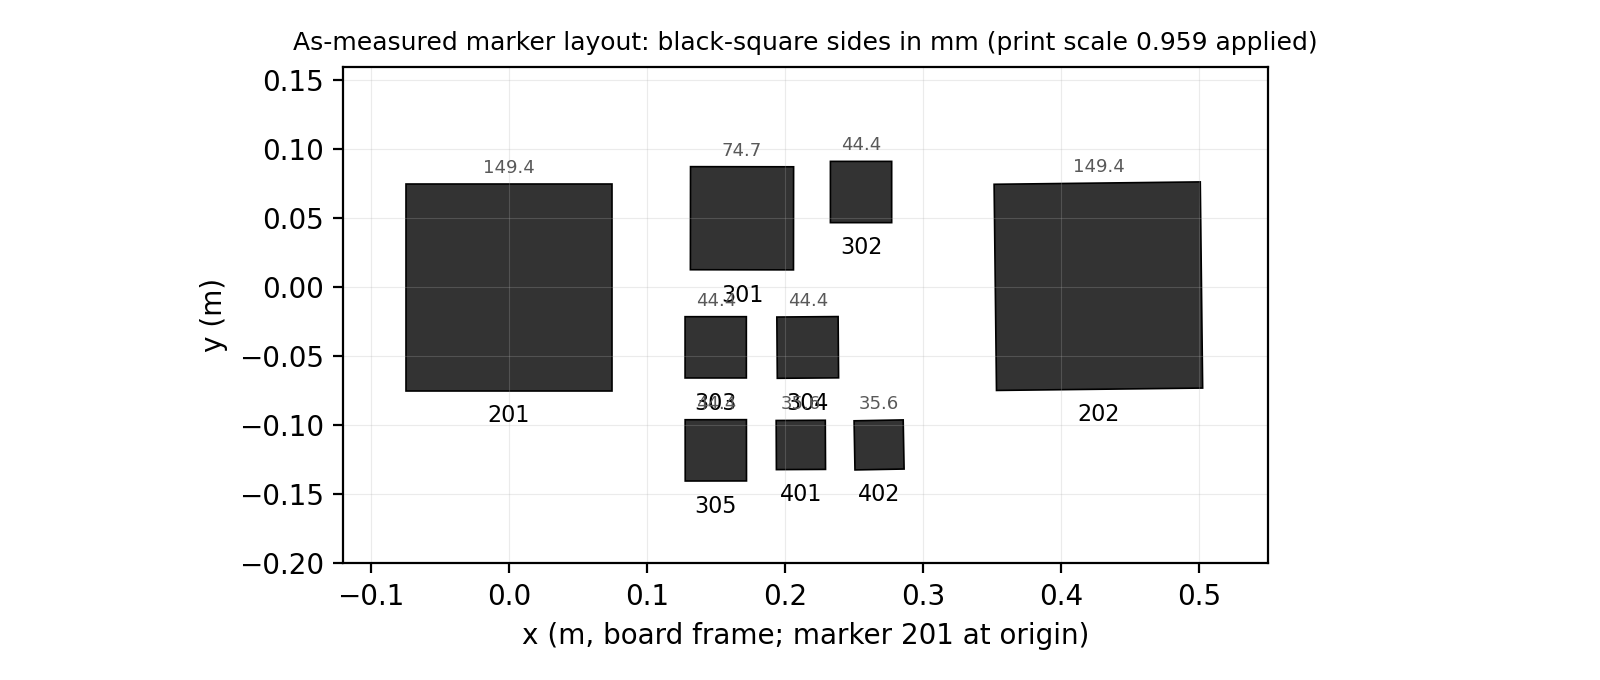
\includegraphics[width=0.85\textwidth]{Figures/board_layout.png}
    \caption{As-measured marker layout in the board frame, positions and
    black-square sides estimated from the data with the 0.959 print scale
    applied. The four size groups placed at a common range are the
    marker-size lever of the experiment.}
    \label{fig:board}
\end{figure}

\subsubsection{Capture setup}

Data was captured in a single pool session with a ZED stereo camera, of
which only the left, rectified stream was recorded (960$\times$540 at
nominal 15~Hz), giving a monocular ArUco problem; images, camera info and
the ZED IMU were logged. Two runs were
recorded: an on-axis walk-back (677 frames at an effective 2.5~Hz over
271~s) and an oblique walk-back from roughly 4~m of lateral offset (737
frames over 85~s, with about 42\% of frames dropped in bursts by disk
bandwidth; the two runs are therefore analysed separately and never
pooled). The vehicle was hand-held and paced backwards from the board to
beyond the detection limit, with a yaw turn at each step.

Camera intrinsics are the shipped in-air factory rectification
($f_x{=}f_y{=}797.5$, zero distortion on the rectified stream). The
in-water validity of this choice was tested by a joint bundle adjustment
over 1400 marker observations in 317 frames, solving for underwater focal
lengths, the coplanar board layout and per-frame poses with scale pinned by
the ruler-measured marker sizes: the aspect ratio solves to
$f_y/f_x = 0.996$ and the isotropic optimum is only 1.9\% better than the
in-air value, while the flat-port refraction correction of $1.333\times$
is rejected outright (44\% worse residual). The shipped intrinsics are
therefore used unchanged, and all metric ranges carry an approximately
$\pm$10\% scale uncertainty from the focal length, which dominates the
error budget. For this reason the primary independent variable throughout
Part~B is the calibration-free \emph{apparent marker size in pixels};
metric range is derived and reported with its uncertainty.

\subsubsection{Experiment design}

The two walk-backs sweep range continuously from about 0.6~m to beyond the
detection limit, and marker size is swept \emph{by construction}: four size
groups (149.4 down to 35.6~mm, a 4.2$\times$ lever) are present on the
board simultaneously, so every frame samples all sizes at a common range
and water condition. Viewing angle was not controlled: the on-axis run has
a median marker incidence of 13$^\circ$ and the oblique run 58$^\circ$,
two disconnected regimes confounded with range and marker size, so no
detection-versus-angle curve is reported.

No external ground truth exists (no tape or survey range, and vehicle
odometry was not recorded); scale is anchored solely by the ruler-measured
marker sizes and attitude solely by an IMU gravity check. Detection is
scored per marker-frame trial against apparent-size bins with a minimum of
ten trials per bin and Wilson confidence intervals (2551 trials on-axis,
950 oblique). Maximum detection range is established uncensored: the
on-axis walk continued for a further 79~s (about 3~m) beyond the last
detection with zero detections, and two independent end-of-run estimates
(walk-back rate extrapolation and board apparent width in the final frame)
agree at 7.8 to 8.1~m, so range limits below are detection failures, not
end-of-data artefacts.

\subsubsection{Turbidity measurement and synthetic degradation}

Water attenuation was measured photometrically from the target itself,
without dosing or a turbidity meter. A black patch (marker border) and a
white patch (surrounding sheet) at the same range share an identical
veiling-light term in the image formation model
$I = J e^{-\beta d} + B(1 - e^{-\beta d})$, so their difference is free of
$B$: $\mathrm{contrast}(d) = (J_w - J_b)\,e^{-\beta d}$, and $\beta$ is a
straight-line fit in log space. Two corrections proved load-bearing: an
instrument-response correction $k$(apparent~px), measured at fixed range so
it is independent of $\beta$, without which small (hence distant-looking)
markers read up to 18\% low and the bias imitates attenuation; and
per-marker intercepts, since the three sheets sit under different local
lighting. The underlying image formation model is the standard
attenuation-plus-veiling form \cite{jaffe1990computer}.

Higher turbidity than the pool's was synthesised by re-attenuating each
real frame in place: $I' = B + (I - B)\,e^{-\Delta\beta\, d(x)}$ per
channel and per pixel, with the per-pixel range $d(x)$ taken from the
board-plane pose and $\Delta\beta = m\,\beta$ for multipliers
$m \in \{0, 0.25, 0.5, 1, 1.5, 2, 3, 4, 6, 8\}$, where $m{=}0$ reproduces
the real frame. Results are reported against total optical depth
$\tau = (1{+}m)\,\beta d$ rather than named water types: range enters the
model only as the product $\beta d$, so any uniform scale error in $d$ is
absorbed into $\beta$, making the $\tau$ axis immune to the $\pm$10\%
range uncertainty and portable across waters and cameras. The synthesis
adds no scattering blur, so any benefit a contrast-enhancing preprocessor
shows on synthesised frames is an upper bound. The full chain is
summarised in Figure~\ref{fig:turbpipe}.

\begin{figure}[H]
\centering
\begin{tikzpicture}[font=\scriptsize, >={Stealth[length=2mm]},
  box/.style={draw, rounded corners=1pt, align=center, minimum height=9mm, inner sep=3pt}]
  \node[box] (frame) {frame};
  \node[box, right=6mm of frame] (warp) {canonical\\marker warp};
  \node[box, right=6mm of warp] (patch) {black ring /\\white surround};
  \node[box, right=6mm of patch] (contrast) {$B$-free contrast\\$(J_w{-}J_b)e^{-\beta d}$};
  \node[box, right=6mm of contrast] (corr) {$k(\mathrm{px})$ +\\fixed effects};
  \node[box, right=6mm of corr] (beta) {$\beta$ per\\channel};
  \node[box, below=8mm of beta] (synth) {re-attenuate:\\$I' = B + (I{-}B)e^{-m\beta d(x)}$};
  \node[box, left=6mm of synth] (sweep) {detection sweep\\(2551 trials $\times$ 10 levels)};
  \node[box, left=6mm of sweep] (env) {envelope:\\rate(px, $\tau$), sizing rule};
  \draw[->] (frame) -- (warp);
  \draw[->] (warp) -- (patch);
  \draw[->] (patch) -- (contrast);
  \draw[->] (contrast) -- (corr);
  \draw[->] (corr) -- (beta);
  \draw[->] (beta) -- (synth);
  \draw[->] (synth) -- (sweep);
  \draw[->] (sweep) -- (env);
\end{tikzpicture}
\caption{Turbidity processing: the top row measures the water's
attenuation from the target itself via the veiling-free contrast; the
bottom row stresses the same real frames to higher optical depth and maps
the detection envelope.}
\label{fig:turbpipe}
\end{figure}

\subsubsection{Detection pipeline and metrics}

Detection uses OpenCV~4.10 with the current \texttt{ArucoDetector} API,
subpixel corner refinement, and \texttt{adaptiveThreshConstant} lowered
from the default 7 to 3, the best of a grid over $\{3, 5, 7\}$ scored at
the highest synthesised turbidity (selected without a holdout, so its
reported rate is an optimistic bound). Single-marker pose, the quantity
under test, uses planar PnP (IPPE square); the reference for
self-consistency is a multi-marker board PnP computed leave-one-out, with
the marker under test excluded from its own reference. Off-board IDs are
deliberately not filtered so the misidentification rate remains
measurable. Reported metrics are detection rate per apparent-size bin and
per derived-range bin, uncensored maximum detection range per marker,
single-marker translation and rotation deviation from the board reference
(self-consistency, not accuracy, since no ground truth exists),
misidentification rate, and an IMU gravity check as the sole
camera-independent attitude validation.


\section{Results and discussion}

% Target ~15-20 pages (largest section -- this is where your contribution lives).
% Mirror Part A / Part B. Interpret results; link back to the gaps and objectives.

\subsection{Part A: Simulation results}
\label{sec:results-a}

\subsubsection{Perception envelope}

The filter's accuracy is governed by range through the $\alpha r^2/s$
measurement noise model. With the vehicle stationary 5~m from the dock the
fused noise floor is approximately 0.11~m and the filter reports
\textsc{degraded} throughout; at 2.2~m the floor drops to approximately
0.02~m, the filter is \textsc{healthy} for 92\% of the run (median position
standard deviation 0.018~m), and the velocity state tracks the true dock
velocity with amplitude ratio 0.85 and correlation 0.89
(Figure~\ref{fig:vel-check}). At the opposite extreme, marker visibility
collapses at contact range: binning fine-alignment health by ground-truth
range shows 84\% to 100\% healthy beyond 5~cm of the entry but only 21\%
inside it, a blackout produced by the large markers overflowing the camera
field of view. This measured envelope, reliable from roughly 2.5~m down to
0.05~m, motivates both the 0.10~m seat criterion and the delegation of the
final centimetres to mechanical capture.

\begin{figure}[H]
    \centering
    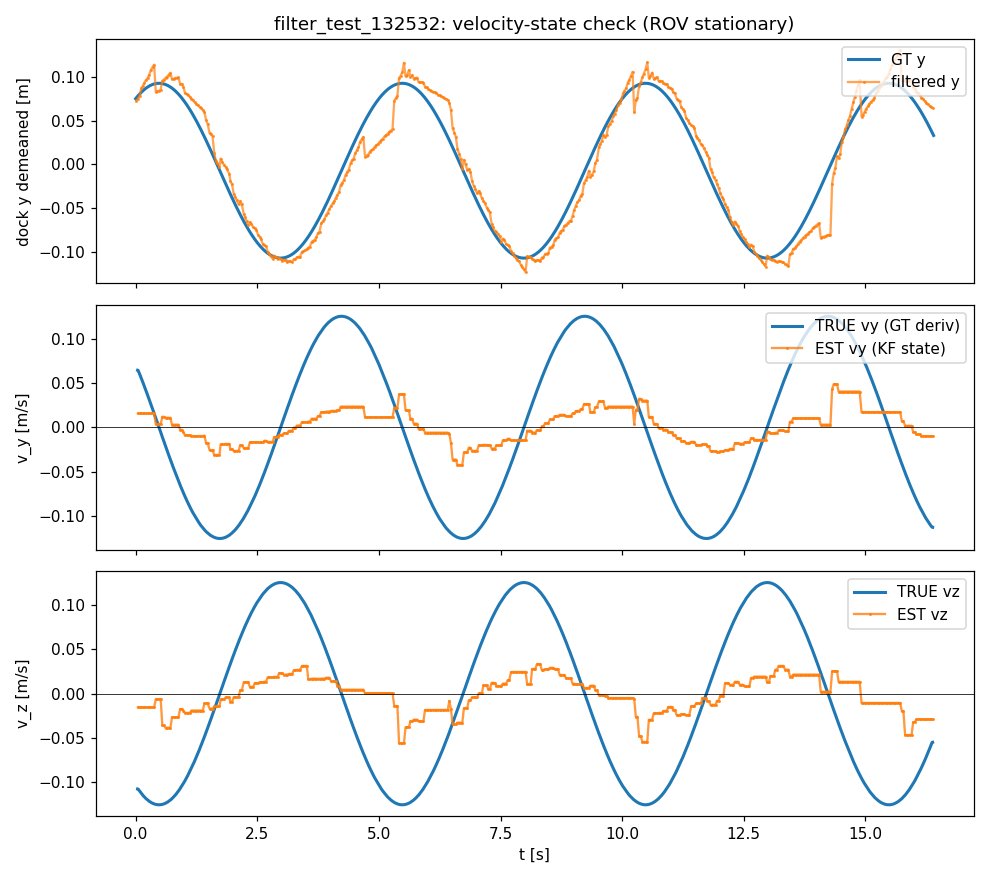
\includegraphics[width=0.85\textwidth]{Figures/vel_check.png}
    \caption{Dock velocity estimation with the vehicle stationary at 2.3~m
    (18~s sway). The velocity state (orange) tracks the ground-truth dock
    velocity (blue) at 0.85 amplitude with correlation 0.89.}
    \label{fig:vel-check}
\end{figure}

\subsubsection{Docking demonstration}

Against the nominal 18~s, 0.1~m orbital sway, the system docks
autonomously end to end: engagement to coarse at $t{+}3$~s, handoff to
fine alignment at $t{+}14$~s, seated and docked at $t{+}25$~s with no
demotions, latching 7 to 8~cm from the entry and coming to rest 4~cm in
front of the dock plane. This trial, and every sweep trial below, ran the
full perception pipeline in the loop with no ground-truth input to the
vehicle.

\subsubsection{Docking envelope versus sway period}

Table~\ref{tab:envelope} and Figure~\ref{fig:pdock} give the headline
result of the sweep ($n{=}3$ per cell, contact-censored scoring). The
baseline (static filter, no feedforward) docks in every trial at every
period in the raw scoring, and cleanly down to 8~s; at 6~s, two of three
trials brush the aperture boundary at low speed (0.03 to 0.06~m/s) before
latching. The method (constant-velocity filter with feedforward) matches
the baseline down to 12~s, degrades at 10~s (one pre-latch contact), and
fails at 8~s and 6~s; its single raw success at 8~s was contact-assisted.

\begin{table}[H]
\centering
\caption{P(dock) by sway period and scoring, $n{=}3$ per cell. Clean
excludes trials with a pre-latch off-aperture crossing.}
\label{tab:envelope}
\begin{tabular}{c|cc|cc}
 & \multicolumn{2}{c|}{Baseline (ff off)} & \multicolumn{2}{c}{Method (CV + ff)} \\
Period [s] & raw & clean & raw & clean \\
\hline
20 & 1.00 & 1.00 & 1.00 & 1.00 \\
16 & 1.00 & 1.00 & 1.00 & 1.00 \\
12 & 1.00 & 1.00 & 1.00 & 1.00 \\
10 & 1.00 & 1.00 & 1.00 & 0.67 \\
8  & 1.00 & 1.00 & 0.33 & 0.00 \\
6  & 1.00 & 0.33 & 0.00 & 0.00 \\
\end{tabular}
\end{table}

\begin{figure}[H]
    \centering
    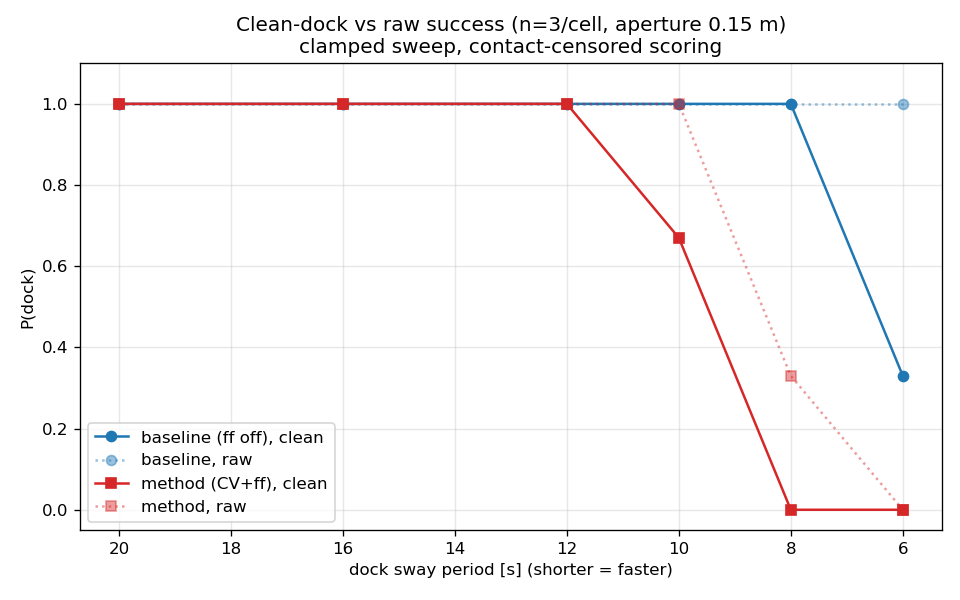
\includegraphics[width=0.8\textwidth]{Figures/clean_pdock.png}
    \caption{Docking success versus sway period under raw (dotted) and
    contact-censored clean (solid) scoring.}
    \label{fig:pdock}
\end{figure}

Clean insertions cross the entry plane 0.003 to 0.05~m off axis at 0.06 to
0.11~m/s closing speed, and all observed contacts occur below 0.06~m/s.
These figures form the interface requirement for a capture mechanism: a
funnel with a capture radius of at least 0.15~m and tolerance for
approximately 0.1~m/s closing speed captures everything the baseline
delivers down to 8~s periods.

\subsubsection{Failure analysis: ego-motion instability of the velocity
estimator}

The method's fast-period failures trace to a single mechanism. The dock
measurement is reconstructed in the world frame through the transform of a
moving camera, so a fraction of the vehicle's own motion leaks into the
measured dock position. This leakage is \emph{correlated with the vehicle
state}, violating the filter's white-noise assumption. The static filter,
with no velocity state, absorbs it as position noise and remains faithful
(estimated sway amplitude 0.7 to 0.9 times truth in all baseline runs). The
constant-velocity filter integrates it into a phantom dock velocity and
extrapolates: estimated amplitude reaches 2.4 to 5 times truth in
successful method runs and 18 to 52 times truth in the failures, where the
estimate has decoupled from the real dock (correlation 0.00 with the true
dock while the estimate's excess motion correlates at 0.88 with the
vehicle's own position). The feedforward closes the loop by injecting the
phantom velocity directly into the command; with the identified plant lag
of approximately 240~ms, the loop gain crosses unity between the 10~s and
8~s periods, which is where the measured cliff sits.

The failure is self-concealing: every alignment signal the system exposes
is computed against its own estimate, and in the failed trials those
signals read seat-tolerance alignment (lateral errors of 0.000 to 0.017~m)
while ground truth shows the vehicle 0.17 to 0.48~m off axis at the dock
plane. Only the ground-truth channel exposes the divergence, an argument
for independent verification in any real deployment.

Three progressively stronger mitigations were evaluated. Bounding the
velocity state at the physical dock speed and adding the covariance
ceiling eliminated the metre-scale runaway and the resulting collisions,
but did not restore fast-period docking. Sweeping the process noise
density $\sigma_a$ over 0.02 to 0.16~m/s$^2$ found no stable setting:
estimated amplitude remained 5 to 37 times truth at every value with no
monotonic trend, because a smaller gain also makes the filter slower to
shed an acquired phantom velocity. The baseline's immunity is structural
rather than a tuning point: its velocity gain is exactly zero, and no
finite gain interpolates to that property while the measurement error
remains correlated with vehicle motion. The conclusion is that dock
velocity feedforward from a world-frame constant-velocity estimator
requires explicit ego-motion compensation, by fusing vehicle odometry into
the filter or estimating in a vehicle-relative frame, identified as future
work.

\subsubsection{Replication}

The sweep was run in full on two hosts (real-time factors 0.6 and 1.0) and
two filter revisions (before and after the velocity bounds). The
baseline's uniform success and the method's cliff between 10~s and 8~s
reproduced in both, indicating the result reflects the estimator design
rather than compute load, hardware or incidental tuning.

\subsection{Part B: Real-CV results}
\label{sec:results-b}

\subsubsection{Detection rate versus marker size and range}

Detection is governed by apparent size in pixels with a sharp floor.
Across all four size groups the rate is zero below 21~px, transitional in
the 21 to 28~px bin (0.21 to 0.59 depending on size), and above 0.85 from
38~px upward (Figure~\ref{fig:det-px}). On the derived metric axis this
maps to overall on-axis rates of 0.93 for the 149.4~mm markers, 0.61 at
74.7~mm, 0.43 at 44.4~mm and 0.29 at 35.6~mm over the swept range. The
oblique run (median incidence 58$^\circ$) detected only the 149.4~mm
markers, at 0.60 overall; the three smaller groups produced zero
detections in 791 trials, indicating that oblique viewing costs roughly
one size class even before the angle reaches the detector's geometric
limits.

\begin{figure}[H]
    \centering
    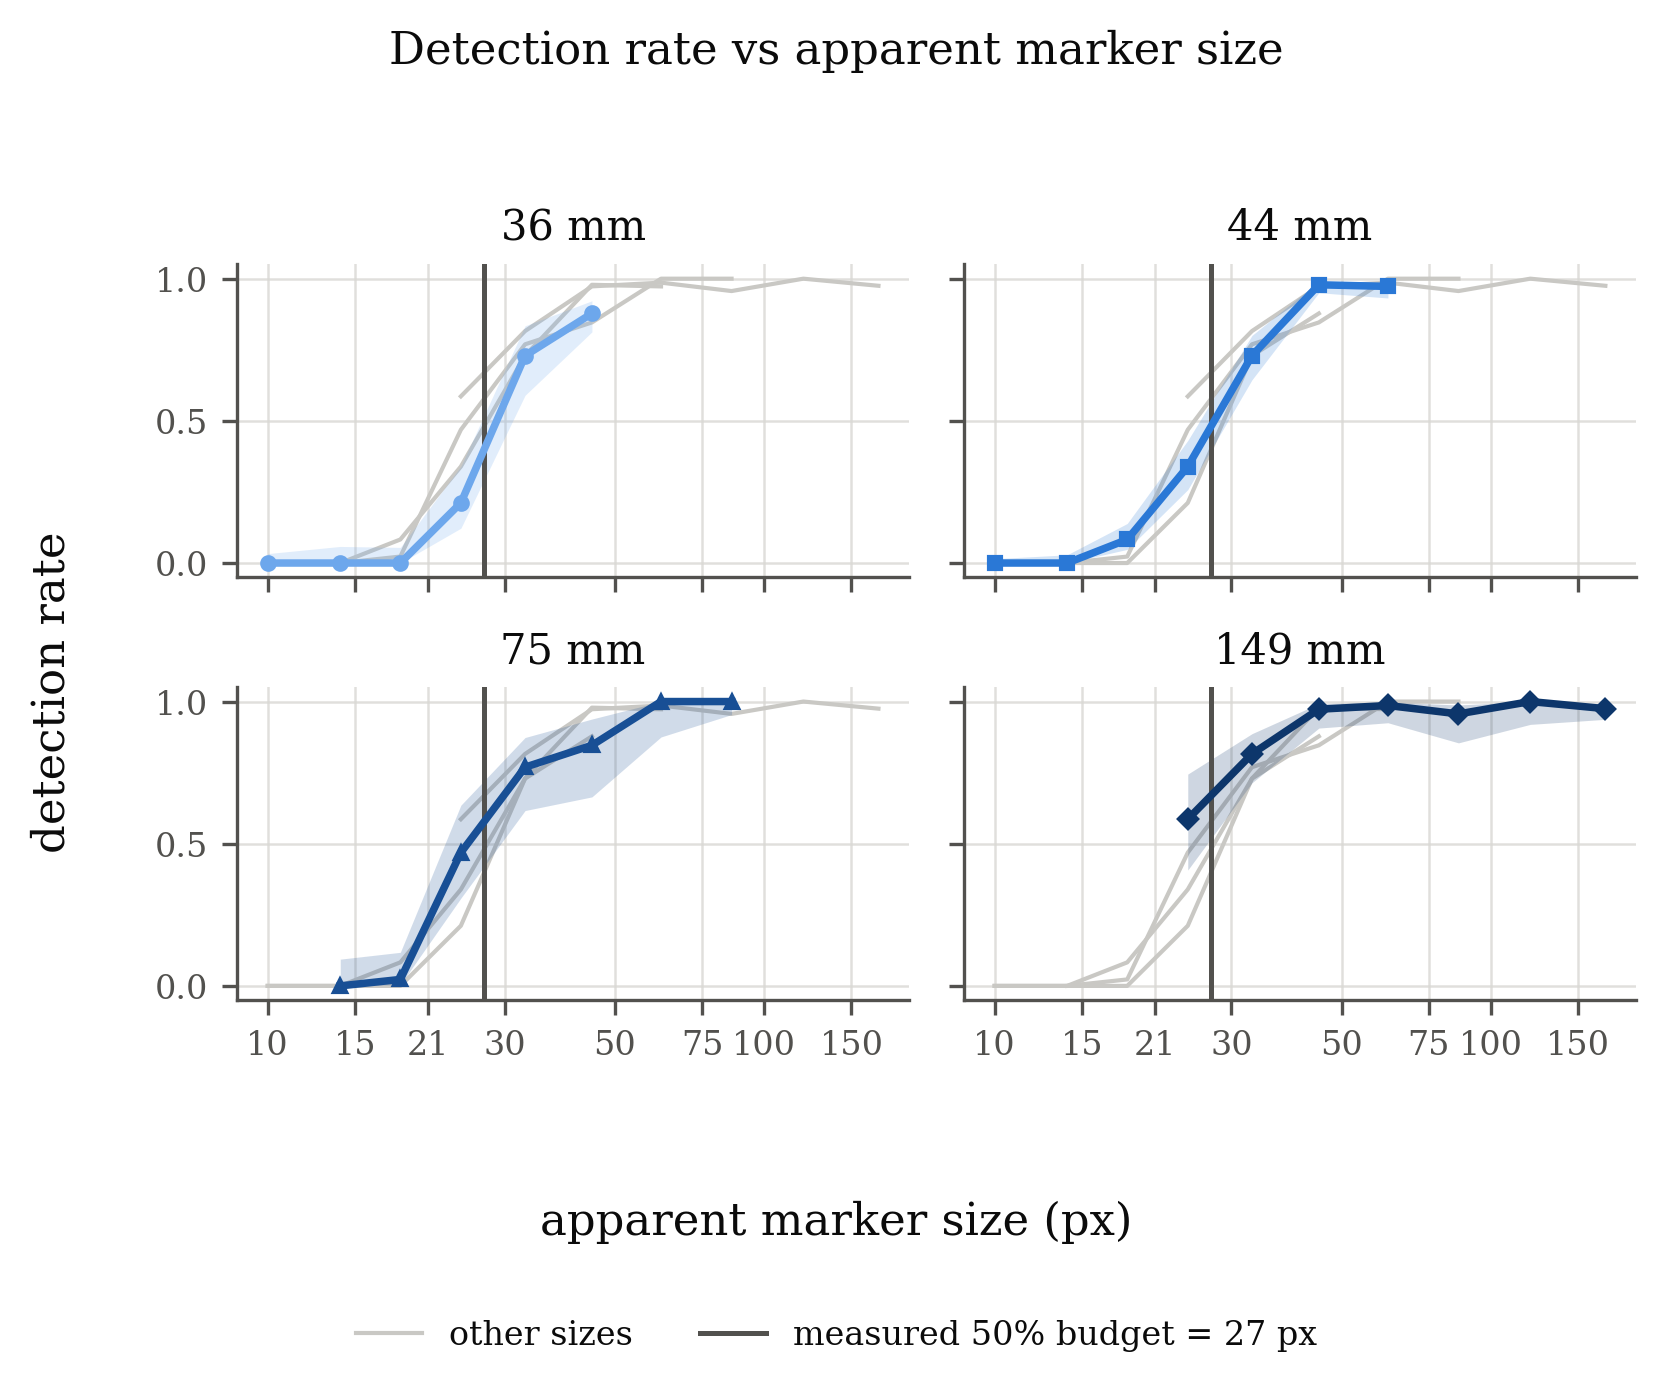
\includegraphics[width=0.95\textwidth]{Figures/detection_rate_vs_px.png}
    \caption{Detection rate versus apparent marker size (pixels), per
    marker size group, with Wilson 95\% intervals; bins with fewer than
    ten trials suppressed. The axis is calibration-free.}
    \label{fig:det-px}
\end{figure}

\subsubsection{Maximum detection range}

Uncensored maximum detection ranges scale linearly with marker side: 5.10
and 4.87~m for the two 149.4~mm markers, 3.05~m at 74.7~mm, 1.55 to
2.17~m at 44.4~mm, and 1.10 to 1.14~m at 35.6~mm, fitted by
$\mathrm{max\ range} \approx 34.9 \times \mathrm{side}$
(Figure~\ref{fig:max-range}). The walk-back continued approximately 3~m
past the last detection with none recorded, so these are genuine detection
limits. Two distinctions matter operationally. First, only the largest
markers reach the 5~m acquisition range assumed for the coarse phase, and
only marginally. Second, maximum range is a single-tail-detection
statistic; the \emph{reliable} (50\%) range sits lower, at 5~m a 149.4~mm
marker subtends 23.8~px, below the $\sim$27~px needed for 50\% detection
(Section~\ref{sec:results-turbidity}), which is why its maximum range of
5.1~m coexists with a 50\% range nearer 4.3~m. Only the second number
sizes a dock.

\begin{figure}[H]
    \centering
    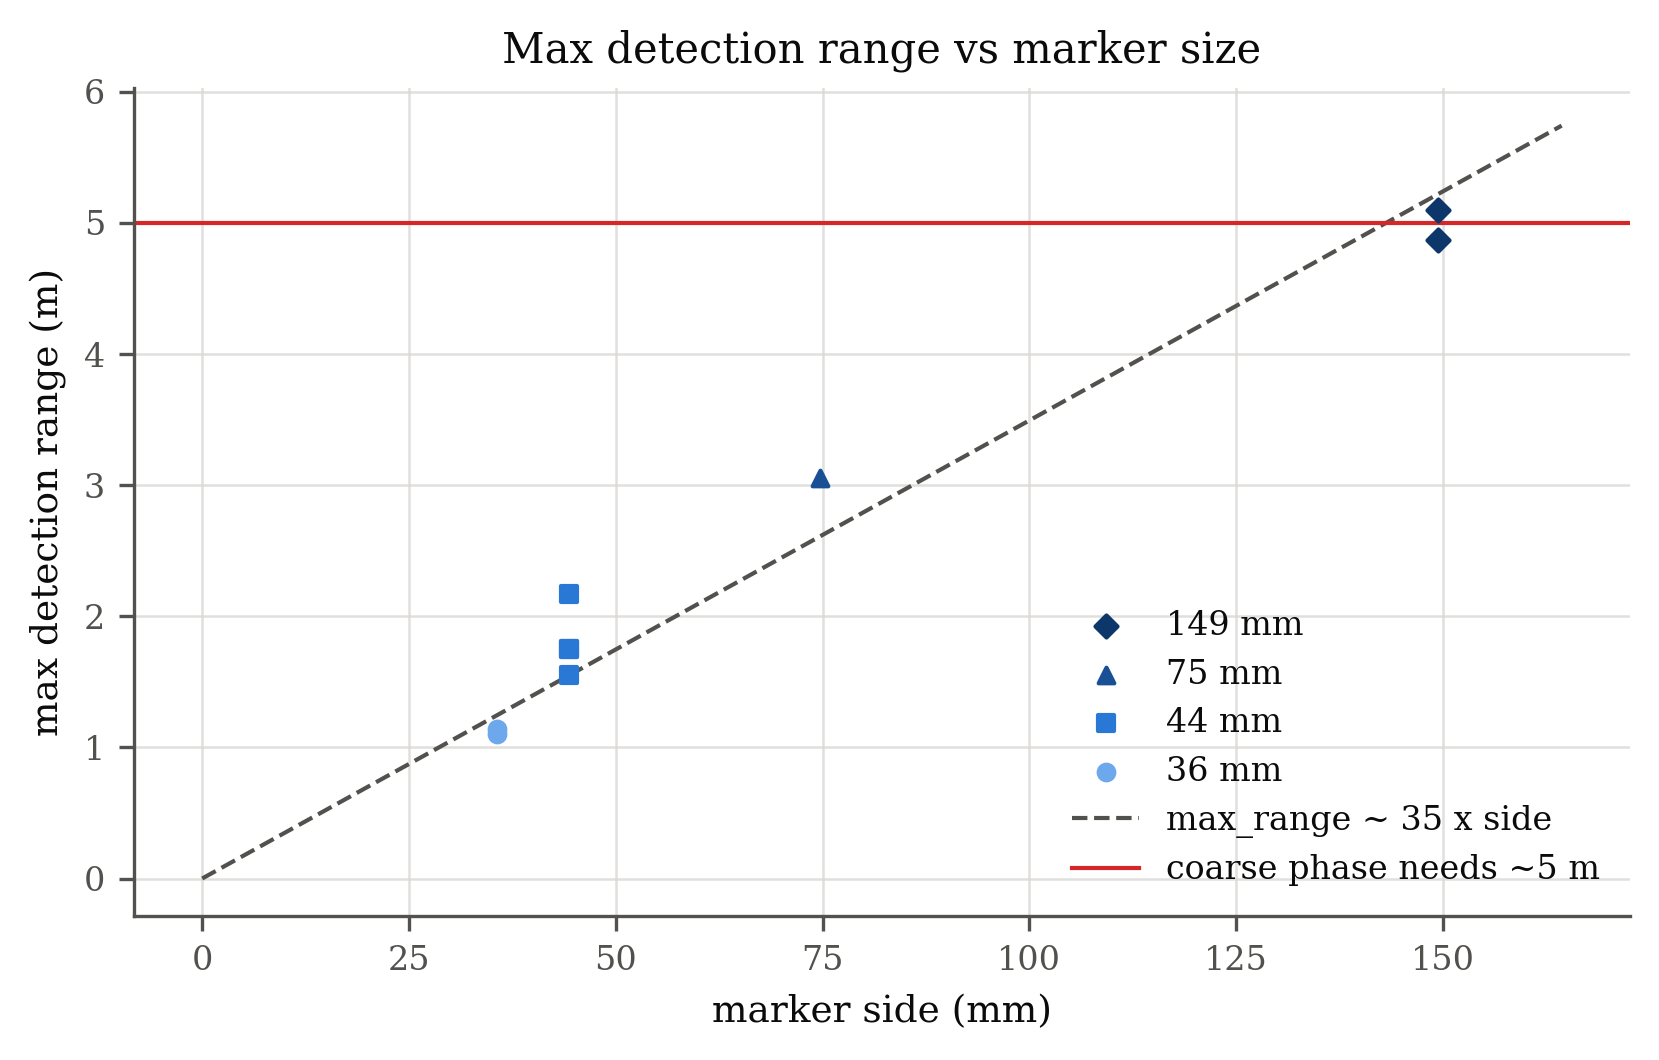
\includegraphics[width=0.8\textwidth]{Figures/max_range_vs_size.png}
    \caption{Maximum detection range versus marker side with the fitted
    linear law and the 5~m coarse-acquisition reference line.}
    \label{fig:max-range}
\end{figure}

\subsubsection{Pose self-consistency and misidentification}

With no external ground truth, single-marker pose is scored against a
leave-one-out multi-marker board reference, a self-consistency measure,
not accuracy. Translation deviation grows from 10.6~mm mean (9.4~mm
jitter) in the 0.5 to 1.0~m bin to 36.1~mm mean (32.9~mm jitter) at 2.0
to 3.0~m; rotation deviation is 11 to 16$^\circ$ and roughly flat with
range. These figures pool all marker sizes, since a per-size split would
change the reference geometry with the marker under test and read
backwards. The sole camera-independent validation is an IMU gravity
check: over 323 frames the board's estimated tilt from vertical has a
median of 6.6$^\circ$, consistent with a hand-held, approximately
vertical board. A yaw-rate cross-check was not corroborative (only 7 of
25 turn segments had sufficient board coverage, and vision magnitudes did
not track the gyro), and is reported as such. Misidentification was
essentially absent in real water: one off-board ID in 1376 on-axis
detections (rate 0.0015) and none in the oblique run.

\subsubsection{Attenuation measurement}

The B-free contrast fit yields, with instrument correction and per-marker
intercepts over 934 samples spanning 0.62 to 3.19~m: $\beta_b = 0.279$,
$\beta_g = 0.247$, $\beta_r = 0.443$, $\beta_{grey} = 0.289$~m$^{-1}$
($r^2 = 0.71$, 0.67, 0.88, 0.75; Figure~\ref{fig:beta}). The strongest
support for the correction chain is a quantity it never saw: the
red-to-green attenuation ratio moves from 1.50 (raw) to 1.79 (corrected),
against approximately 1.8 expected from water optics. A residual check
over 5629 near-to-far marker pairs (not a statistical cross-validation,
no holdout was used) shows the exponential form predicts real far-frame
contrast to a median error of $-3.1$\% corrected, versus $+18.5$\% raw.
At 5~m this water gives a grey optical depth $\tau = 1.44$, i.e.\ 23.6\%
of contrast surviving. The fitted veiling light $B$ is explicitly not
physically meaningful (negative $r^2$; the green estimate exceeds the
white sheet's own brightness): the method is built so that $B$ cancels
from contrast, and $B$ enters the synthesis only as a DC term that
adaptive thresholding rejects.

\begin{figure}[H]
    \centering
    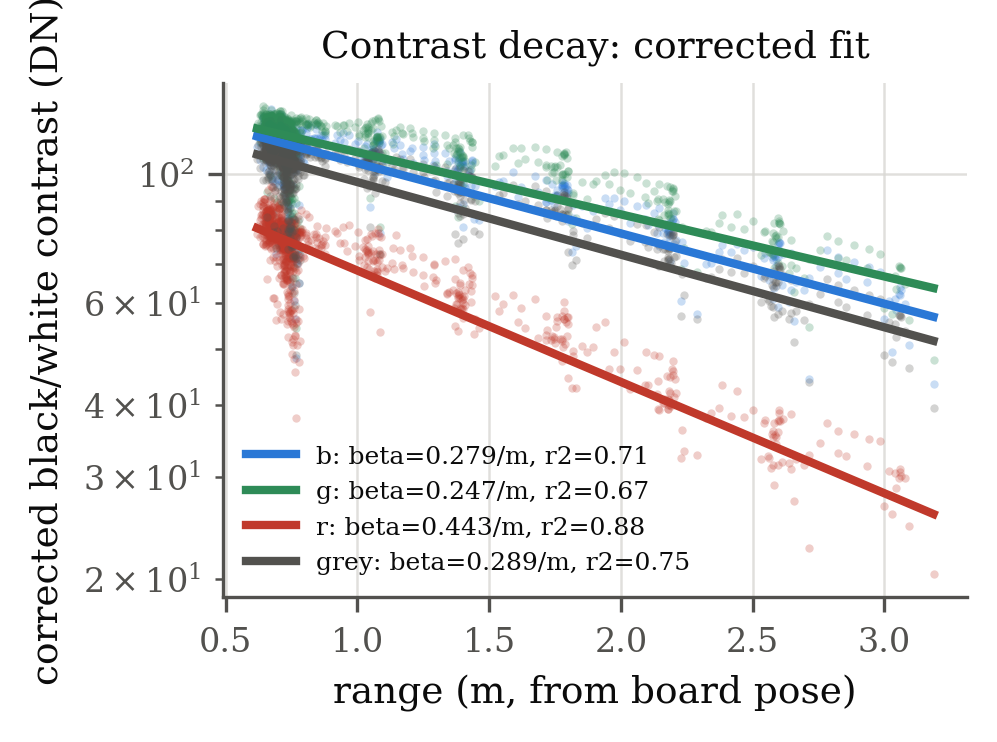
\includegraphics[width=0.8\textwidth]{Figures/beta_contrast_decay.png}
    \caption{Instrument-corrected black-to-white contrast versus range
    with the fixed-effects exponential fits per channel.}
    \label{fig:beta}
\end{figure}

\subsubsection{Turbidity envelope and marker sizing}
\label{sec:results-turbidity}

Re-attenuating all 2551 on-axis trials at ten turbidity multipliers (a
fixed denominator at every level) maps the detection envelope over
apparent size and total optical depth (Figure~\ref{fig:surface}). The
envelope has two regimes: below $\tau \approx 2$ the boundary is
vertical, detection is \emph{pixel-limited} and turbidity hardly moves
it; above $\tau \approx 2.3$ the boundary is horizontal, detection
collapses at every apparent size sampled, \emph{turbidity-limited}. The
pixel budget quantifies the first regime: the apparent size needed for
50\% detection is 27.3 to 28.1~px, flat across a sevenfold span of
optical depth ($\tau$ 0.18 to 1.30), rising only within the resolution of
the binning before the collapse (Figure~\ref{fig:pxbudget}). Two
conclusions follow: the textbook budget of $3(n{+}2) = 21$~px for a
5$\times$5 marker underestimates the real requirement by about 30\%,
because it is a pure sampling argument that assumes air; and ArUco's
adaptive thresholding makes detection remarkably insensitive to contrast
loss until an abrupt threshold near $\tau \approx 2$, a cliff, not a
gradient.

\begin{figure}[H]
    \centering
    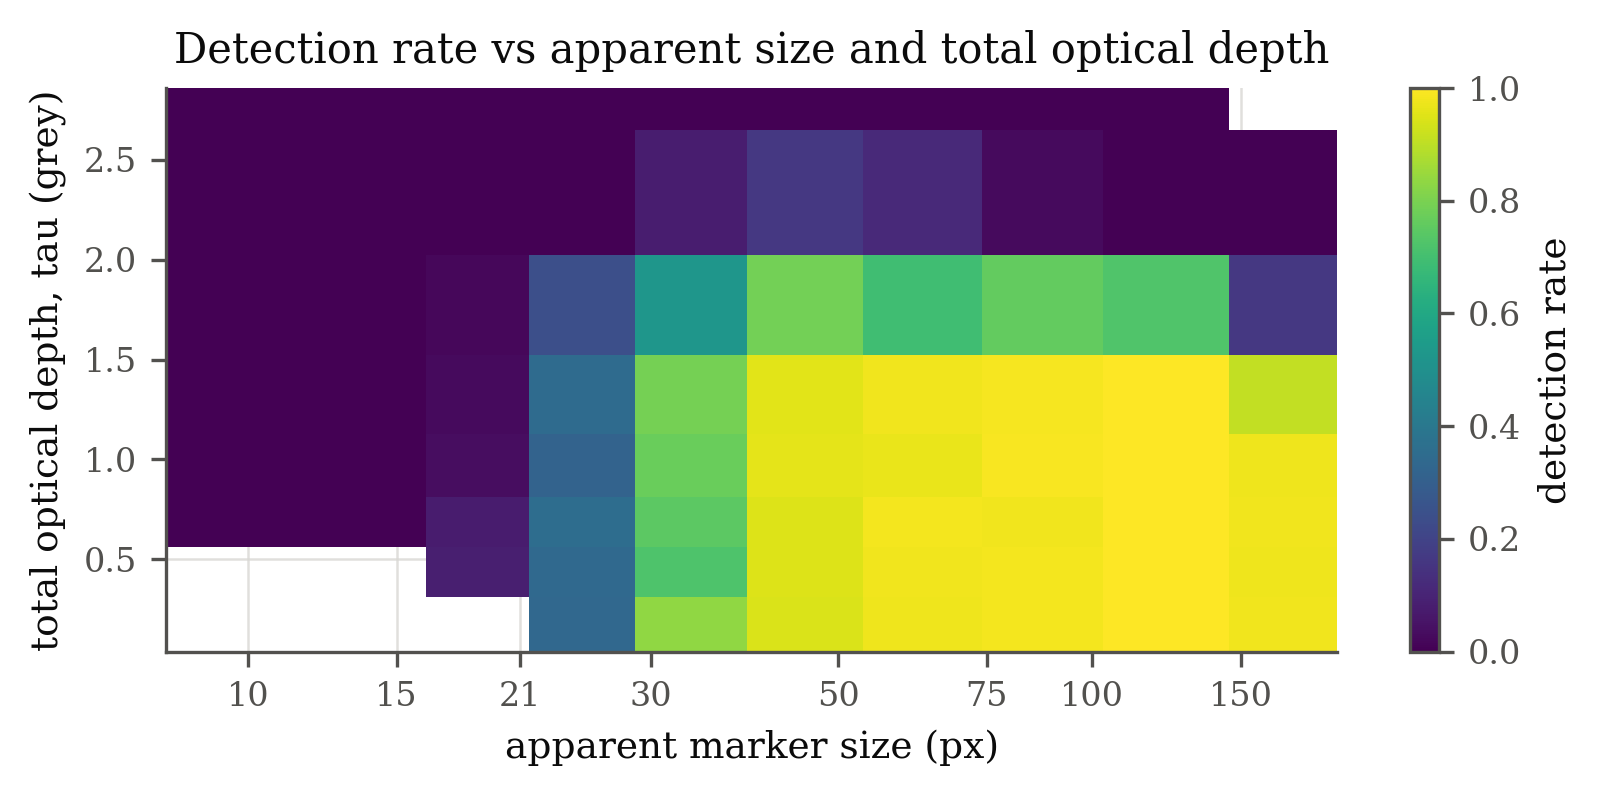
\includegraphics[width=0.9\textwidth]{Figures/rate_px_tau_surface.png}
    \caption{Detection rate over apparent size and total optical depth.
    The boundary is vertical (pixel-limited) below $\tau \approx 2$ and
    horizontal (turbidity-limited) above. White cells are physically
    unreachable combinations.}
    \label{fig:surface}
\end{figure}

\begin{figure}[H]
    \centering
    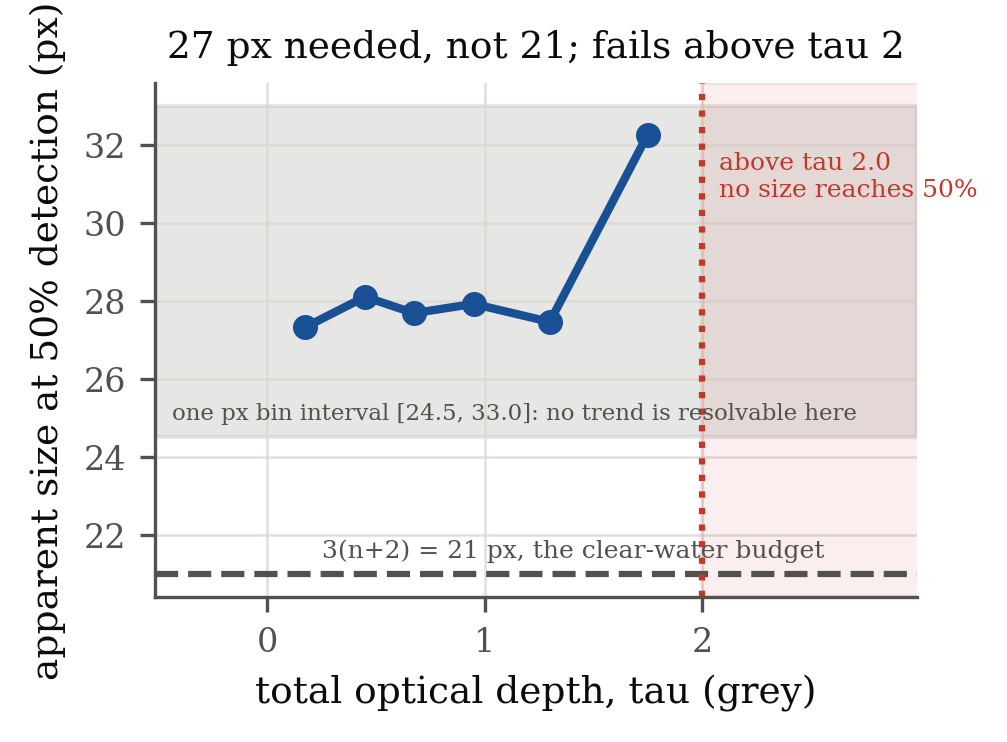
\includegraphics[width=0.8\textwidth]{Figures/px_required_vs_tau.png}
    \caption{Apparent size required for 50\% detection versus optical
    depth: flat at $\sim$27~px across $\tau$ 0.18 to 1.30 (band shows the
    bin-interpolation resolution), undefined above $\tau \approx 2$ where
    no size sampled reaches 50\%.}
    \label{fig:pxbudget}
\end{figure}

Inverting the pixel budget through the pinhole model sizes the dock
marker: for 50\% single-frame detection this pool's water requires a
105~mm marker at 3~m and 182~mm (interval 154 to 207~mm) at 5~m. In
clearer water ($\beta = 0.15$~m$^{-1}$) the 5~m requirement barely drops
(174~mm), confirming that below the cliff the requirement is set by
pixels, not water; in murkier water ($\beta \geq 0.6$~m$^{-1}$, $\tau
\geq 1.8$ at 3~m) the requirement is undefined within the measured
envelope, no marker size sampled achieves 50\%. The textbook 21~px budget
would have specified 132~mm at 5~m, 38\% short in side length and roughly
half the area. The synthesised degradation is illustrated in
Figure~\ref{fig:strip}; a forward-scatter check found no measurable edge
blurring within apparent-size bins across the synthesised range
(slopes scatter around zero), so at these optical depths contrast loss,
not blur, is the operative mechanism.

\begin{figure}[H]
    \centering
    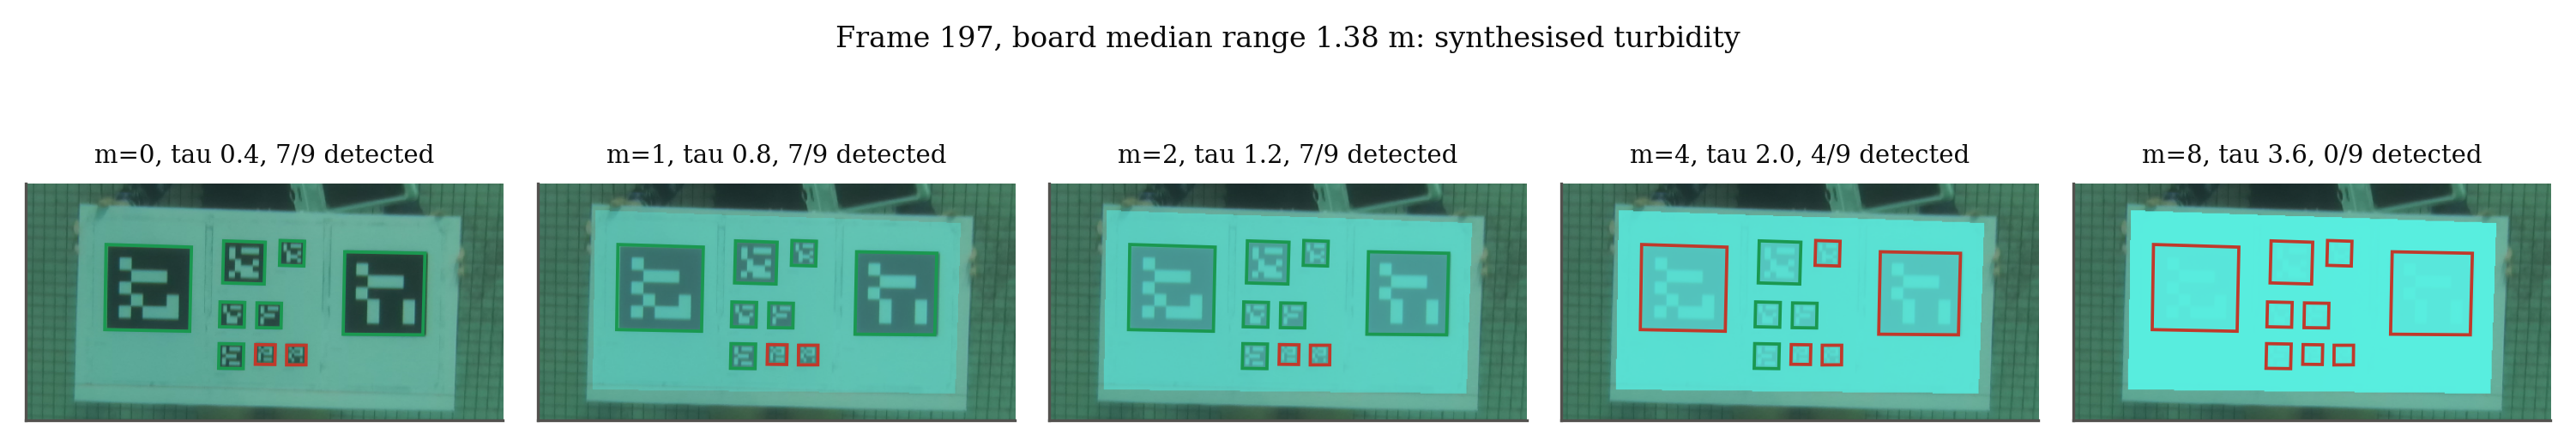
\includegraphics[width=0.95\textwidth]{Figures/synthesis_sweep_strip.png}
    \caption{One frame re-attenuated at increasing turbidity multipliers
    with detections outlined: 7 of 9 markers at the real condition
    falling to 0 of 9 at the highest multiplier. The highest-multiplier
    panel is a diagnostic of the synthesis (its DC term is unphysical),
    not a depiction of real murky water.}
    \label{fig:strip}
\end{figure}

\subsubsection{Preprocessing: CLAHE evaluated and rejected}

CLAHE was evaluated against the detector's own thresholding knob over all
2551 trials at every turbidity level. In \emph{real} water (multiplier 0)
CLAHE is a net negative: detection 0.512 versus 0.519 baseline, while
introducing 0.022 misidentifications per frame where the baseline has
zero. Its apparent gain at high synthesised turbidity (0.337 versus 0.159
at the highest level) is measured on frames whose degradation adds no
scattering noise, and is therefore an upper bound unproven for real
water. Lowering \texttt{adaptiveThreshConstant} to 3 recovers about
two-thirds of that gap (0.276) at a third of CLAHE's misidentification
rate (Figure~\ref{fig:preproc}). The engineering decision follows the
real-water evidence: no CLAHE stage in the pipeline; tune the detector's
threshold constant instead.

\begin{figure}[H]
    \centering
    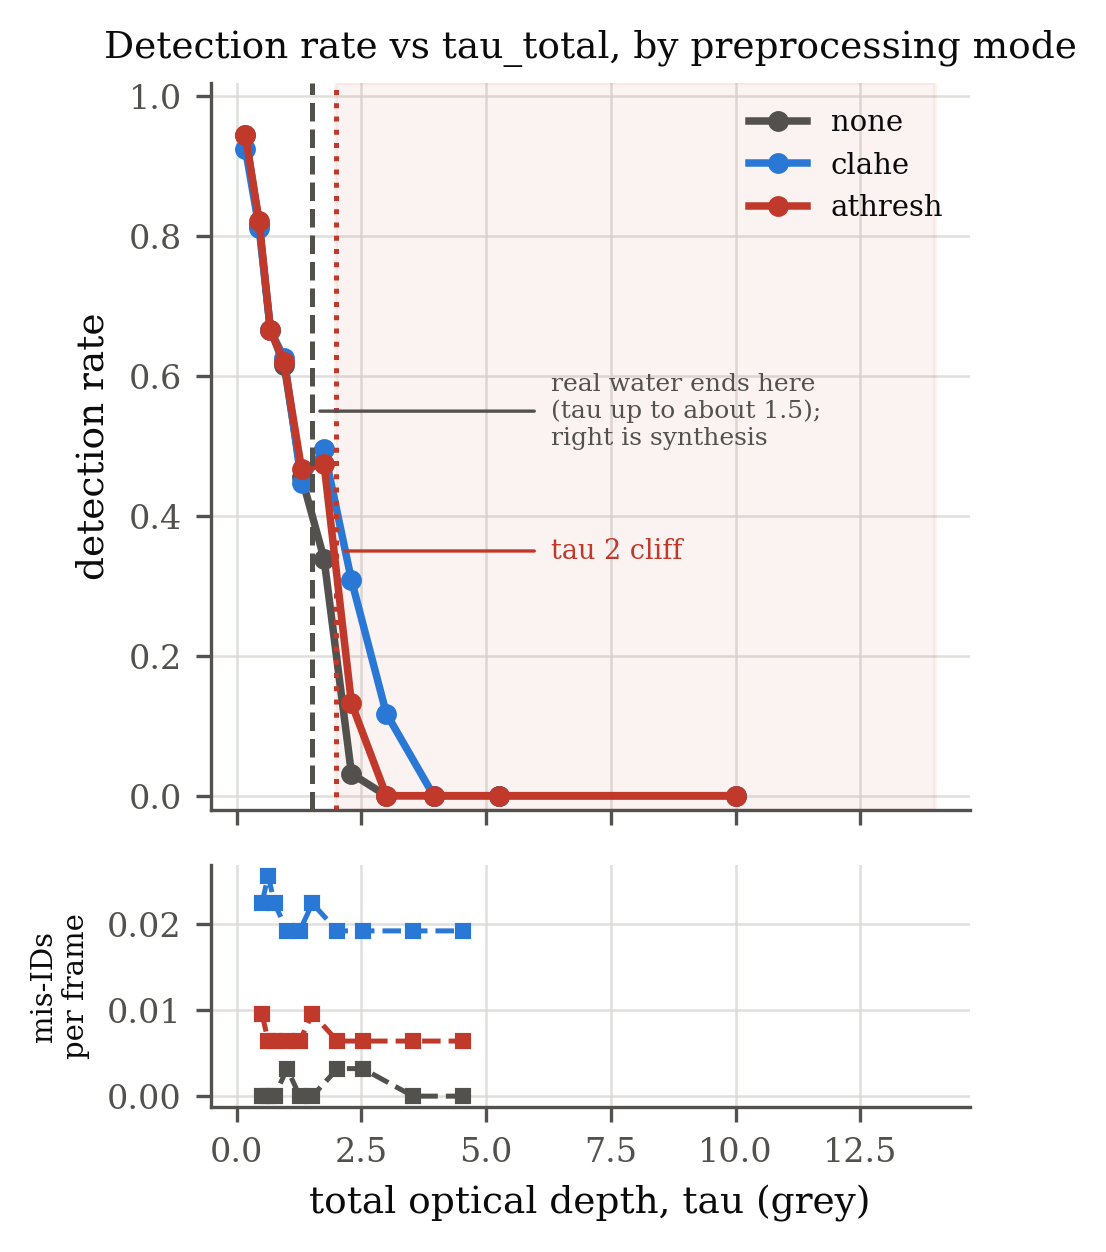
\includegraphics[width=0.9\textwidth]{Figures/preprocessing_eval.png}
    \caption{Detection rate (top) and misidentifications per frame
    (bottom) versus total optical depth for no preprocessing, CLAHE, and
    a lowered adaptive-threshold constant. Real water ends at the dashed
    line; everything beyond is synthesised.}
    \label{fig:preproc}
\end{figure}

\subsubsection{Limitations}

The dataset is one pool, one session: the optical-depth axis is designed
to generalise (results are reported against $\tau = \beta d$), but this
water is a single point and the attenuation spectrum of other waters will
differ. No external ground truth exists; pose results are
self-consistency only, and all metric ranges carry $\pm$10\% from the
in-air focal length. $\beta$ was fitted over 0.62 to 3.19~m, so quoting
$\tau$ at 5~m assumes $\beta$ constant with range. The oblique run is
thin (161 detections, largest markers only) and viewing angle was never
controlled. The capture was hand-held, so motion blur is present and
unmodelled, and synthesised turbidity levels derive from the same frames
and are correlated samples, so the quoted confidence intervals understate
uncertainty at high multipliers.

\subsection{Synthesis}

The two halves bound the operating envelope of passive-marker terminal
docking from opposite sides. Part~A bounds the \emph{dynamics}: with the
full perception pipeline in the loop, the vehicle captures a swaying dock
cleanly down to 8~s periods at 0.1~m amplitude, limited by its own
control bandwidth (240~ms plant lag), and delivers insertions a capture
funnel of 0.15~m radius and 0.1~m/s tolerance can accept. Part~B bounds
the \emph{sensing}: a marker is reliably detectable only above
$\sim$27~px of apparent size and below $\tau \approx 2$ of optical
depth, which in the measured water prices the 5~m acquisition range at a
182~mm marker (154 to 207~mm) and rules out reliable acquisition at that
range in substantially murkier water regardless of size.

The intersection is the design statement for the dock. The 200~mm-class
markers assumed throughout Part~A are validated by Part~B as marginally
sufficient for 5~m acquisition in pool-clarity water, with the
per-size fusion pipeline of Part~A consuming exactly the size-dependent
envelope Part~B measured (small markers taking over as large ones
overflow the field of view at close range, whose 5~cm blackout sets the
seat criterion). Beyond the measured envelope, at longer standoff or
higher turbidity, the passive-marker channel provides no signal, and
terminal docking must be handed a vehicle already inside the envelope by
a far-field cue such as an active light beacon, which is precisely the
acquisition stage this work scoped out and now quantifies the need for.
% TODO expand: one paragraph tying the failure analysis (ego-motion) to the
% deployment recommendation (vehicle-relative estimation), and one on the
% descoped physical docking trials with this envelope as the justification.


\section{Conclusion}
\label{sec:conclusion}

This thesis built and validated the terminal stage of underwater docking using passive markers and classical computer vision, the approach available to low-cost platforms. The system consists of multi-marker ArUco fusion, an error-state Kalman filter with two dock-motion models, and a coarse-to-fine docking state machine. The full perception pipeline runs in the loop, and the vehicle never receives ground truth.

In simulation, the system docks onto a moving target. The baseline configuration docked at every sway period down to 8~s at 0.1~m amplitude, which covers moored docks at typical continental-shelf depths in the mean New South Wales sea state. The velocity feedforward fails at short periods because the vehicle's own motion leaks into the dock measurement and is integrated into a phantom dock velocity. Tuning cannot fix this failure, the system's own health signals cannot see it, and the baseline is immune because it never estimates velocity.

On real underwater imagery, detection needs about 27 pixels of apparent marker size, and the maximum detection range is about 35 times the marker side. Detection collapses once the total optical depth exceeds about 2. In the measured pool water, these numbers set the marker for 5~m acquisition at 182~mm (154 to 207~mm).

Together, the two parts bound where this class of system works, from the motion side and from the sensing side. They also supply the numbers a dock designer needs, namely a capture funnel of at least 0.15~m radius tolerating about 0.1~m/s closing speed, and the marker sizing rule above. Both quantities come from measurement. In addition, no stage of the pipeline depends on a trained model, so the measured limits are properties of the approach itself.

\subsection{Future work}
\label{sec:future-work}

The first priority is to fix the velocity estimator. It breaks because the dock measurement is built through the vehicle's own pose, so the vehicle's motion ends up inside the measurement. There are two ways to remove this. The filter could take in the vehicle odometry, so it knows which part of the motion belongs to the vehicle. Alternatively, the dock could be estimated directly relative to the vehicle, so the vehicle's world position is never involved. Either fix should be tested against the same sway sweep, and it still has to work with the 240~ms lag, since the instability appears once the lag becomes large compared to the sway period.

The natural next step is hardware testing with the combined work of Part~A and Part~B. Part~B measured the camera side in an open loop, while Part~A closed the loop only in simulation. A pool trial with the real BlueROV2, the printed marker board and the full docking stack would test both halves together for the first time. The 240~ms lag should be measured again on the real vehicle early on, since the failure period can be predicted from it before any docking is attempted.

On the measurement side, the camera should be calibrated underwater. This would remove the $\pm$10\% range uncertainty that dominates Part~B's error budget, since the metric ranges and the marker sizing rule would then rest on a measured focal length instead of the in-air factory value.

The detection measurements should also be repeated in genuinely turbid water. The synthetic turbidity adds contrast loss but no scattering blur, so the high-turbidity results are an upper bound. A repeat in a dosed and isolated tank or a naturally murky site would show whether the $\sim$27~px budget and the $\tau \approx 2$ cliff still hold with real scattering.

Finally, a sway-aware dock motion model may recover the feedforward benefit without the ego-motion problem. The dock moves in a nearly perfect sine at one wave period, so a model built for that motion is much more constrained than a general constant-velocity model. A more constrained model is harder to corrupt with motion that does not look like a sine, though this remains to be shown against the same sweep.


\cleardoublepage

\addcontentsline{toc}{section}{References}
% The reference list is defined here
\bibliographystyle{plain} % The bibliography style is defined here. A list of avaliable styles can be found here: https://www.overleaf.com/learn/latex/bibtex_bibliography_styles
\bibliography{References} % The reference list is inserted here from the References.bib file

% Reference examples kept for format guidance; delete before submission:
% \input{Sections/Reference Examples}

\section*{Appendix: dock pose measurement and filter formulation}
\addcontentsline{toc}{section}{Appendix: dock pose measurement and filter formulation}
\label{sec:appendix}

This appendix records the perception components that were modified from their published forms, as implemented in the released code. The standard error-state machinery (quaternion error composition, inject and reset) follows Sol\`a \cite{sola2017quaternion} and is not rederived. Quaternion products are written $\otimes$, $R(q)$ is the rotation matrix of quaternion $q$, and $\mathrm{Log}(\cdot)$ maps a quaternion to its rotation vector.

\subsection*{A.1 Per-marker dock pose and measurement noise}

Each detected marker $i$ yields a PnP pose $(\mathbf{p}_i^{c}, q_i^{c})$ in the camera frame. With the marker's surveyed pose in the dock frame $(\mathbf{p}_i^{d}, q_i^{d})$ known from the layout, the dock origin implied by that single marker is
\begin{equation}
    q_{\mathrm{dock},i}^{c} = q_i^{c} \otimes (q_i^{d})^{-1}, \qquad
    \mathbf{p}_{\mathrm{dock},i}^{c} = \mathbf{p}_i^{c} - R\!\left(q_{\mathrm{dock},i}^{c}\right)\mathbf{p}_i^{d}.
\end{equation}

The measurement noise assigned to marker $i$ follows the PnP error scaling, in which position error grows as $r^2/(s f_{px})$ for range $r$, marker side $s$ and focal length $f_{px}$, while rotation error, set by angular rather than metric resolution, carries one factor of $r$ less. With the fixed camera intrinsics absorbed into a single calibrated constant $\alpha$,
\begin{equation}
    \sigma_{p,i} = \alpha\, r_i^2 / s_i, \qquad
    \sigma_{R,i} = \alpha\, r_i / s_i, \qquad
    \mathbf{R}_i = \mathrm{diag}\!\left(\sigma_{p,i}^2 \mathbf{I}_3,\; \sigma_{R,i}^2 \mathbf{I}_3\right),
\end{equation}
with $\alpha = 0.001$ in all Part~A trials. This range-squared kernel replaces the exponential weight of Xu et al.\ \cite{xu2021underwater}, which saturates numerically once $r/s$ leaves its calibrated band and the quadratic form grows without bound at far range, which is physically correct and handled downstream by the validation gate.

\subsection*{A.2 Spatial consensus}

Before fusion, the implied dock orientations are checked for mutual consistency following the spatial outlier test of Kim et al.\ \cite{kim2024enhancing}. For each pair $(i,j)$ the geodesic rotation distance $\theta_{ij} = \left\| \mathrm{Log}\!\left((q_{\mathrm{dock},i}^{c})^{-1} \otimes q_{\mathrm{dock},j}^{c}\right) \right\|$ is compared against a threshold of $8^{\circ}$. Each marker's disagreement count is the number of pairings exceeding the threshold, and the worst marker is removed iteratively until all survivors agree. The test is skipped when fewer than three markers are visible, since no majority exists.

\subsection*{A.3 Inverse-variance fusion}

The surviving single-marker poses are fused by inverse-variance weighting \cite{xu2021underwater}. Position fuses in closed form,
\begin{equation}
    \mathbf{P}_p = \Bigl(\textstyle\sum_i \sigma_{p,i}^{-2}\mathbf{I}_3\Bigr)^{-1}, \qquad
    \hat{\mathbf{p}} = \mathbf{P}_p \textstyle\sum_i \sigma_{p,i}^{-2}\,\mathbf{p}_{\mathrm{dock},i}^{c},
\end{equation}
and orientation fuses by the same weights in the tangent space at the first survivor's quaternion $q_1$. With $\boldsymbol{\delta}_i = \mathrm{Log}(q_1^{-1} \otimes q_{\mathrm{dock},i}^{c})$,
\begin{equation}
    \mathbf{P}_R = \Bigl(\textstyle\sum_i \sigma_{R,i}^{-2}\mathbf{I}_3\Bigr)^{-1}, \qquad
    \hat{q} = q_1 \otimes \mathrm{Exp}\Bigl(\mathbf{P}_R \textstyle\sum_i \sigma_{R,i}^{-2}\boldsymbol{\delta}_i\Bigr),
\end{equation}
valid to first order because the consensus test bounds the tangent deltas. The fused pose, its covariance and the surviving marker count form the measurement passed to the filter.

\subsection*{A.4 Error-state Kalman filter}

The filter state is $\mathbf{x} = [\mathbf{p}, \mathbf{v}, \boldsymbol{\delta\theta}] \in \mathbb{R}^9$, holding the dock position, the dock velocity and a small-angle rotation error about a reference quaternion $q_{\mathrm{ref}}$ carried alongside the state \cite{sola2017quaternion}. The prediction at rate 30~Hz is constant-velocity in position and identity in rotation,
\begin{equation}
    \mathbf{p} \leftarrow \mathbf{p} + \mathbf{v}\,\Delta t, \qquad
    \mathbf{F} = \begin{bmatrix} \mathbf{I}_3 & \Delta t\,\mathbf{I}_3 & \mathbf{0} \\ \mathbf{0} & \mathbf{I}_3 & \mathbf{0} \\ \mathbf{0} & \mathbf{0} & \mathbf{I}_3 \end{bmatrix}, \qquad
    \mathbf{P} \leftarrow \mathbf{F}\mathbf{P}\mathbf{F}^{T} + \mathbf{Q}.
\end{equation}

The two process-noise regimes of the Part~A ablation differ only in $\mathbf{Q}$. The \emph{static} regime is a position random walk with the velocity block zeroed,
\begin{equation}
    \mathbf{Q}_{\mathrm{static}} = \mathrm{diag}\!\left(q_p \Delta t\,\mathbf{I}_3,\; \mathbf{0}_3,\; q_R \Delta t\,\mathbf{I}_3\right), \qquad q_p = q_R = 10^{-4},
\end{equation}
while the \emph{sway} regime is white-noise acceleration of density $\sigma_a$ (nominally $0.16$~m/s$^2$) with the standard coupled blocks per axis,
\begin{equation}
    \mathbf{Q}_{\mathrm{sway}} =
    \begin{bmatrix}
        \sigma_a^2 \frac{\Delta t^3}{3} \mathbf{I}_3 & \sigma_a^2 \frac{\Delta t^2}{2} \mathbf{I}_3 & \mathbf{0}                  \\
        \sigma_a^2 \frac{\Delta t^2}{2} \mathbf{I}_3 & \sigma_a^2 \Delta t\, \mathbf{I}_3           & \mathbf{0}                  \\
        \mathbf{0}                                   & \mathbf{0}                                   & q_R \Delta t\, \mathbf{I}_3
    \end{bmatrix}.
\end{equation}

The fused measurement observes position and orientation directly, $\mathbf{H} = [\mathbf{I}_3\; \mathbf{0}\; \mathbf{0};\; \mathbf{0}\; \mathbf{0}\; \mathbf{I}_3]$, with innovation $\mathbf{y} = [\hat{\mathbf{p}} - \mathbf{p},\; \mathrm{Log}(q_{\mathrm{ref}}^{-1} \otimes \hat{q})]$ and the fused blocks as $\mathbf{R}$. An update is accepted only if it passes the validation gate
\begin{equation}
    d^2 = \mathbf{y}^{T}\left(\mathbf{H}\mathbf{P}\mathbf{H}^{T} + \mathbf{R}\right)^{-1}\mathbf{y} \;\leq\; \chi^2_{6,\,0.995} = 18.55,
\end{equation}
after which the error state is injected and reset in the usual way \cite{sola2017quaternion}. Two physically motivated bounds close the estimator. After each update the velocity state is clamped isotropically to the maximum credible dock speed, $\mathbf{v} \leftarrow \mathbf{v} \cdot \min(1, v_{\max}/\|\mathbf{v}\|)$ with $v_{\max} = 0.2$~m/s, since a measurement implying a faster dock is ego-motion leakage and not dock motion. A covariance ceiling declares the estimate stale once the position uncertainty exceeds 0.15~m (Appendix~A.5), so controllers hold rather than act on an unconstrained state. Initialisation requires at least two consensus-surviving markers, since a single planar marker leaves the PnP flip ambiguity unresolved. The first accepted measurement seeds the state with its covariance inflated $100\times$, and the initial velocity standard deviation is $0.2$~m/s in the sway regime and $0$ in the static regime.

The static regime is algebraically a constant-position filter. With $\mathbf{v}(0) = \mathbf{0}$, zero initial velocity covariance and zero velocity process noise, every term that could grow the velocity covariance or its cross-covariance with position is zero, so both remain identically zero. The Kalman gain rows onto the velocity state are therefore zero for every update, and $\mathbf{v} \equiv \mathbf{0}$ for all time. The baseline of Part~A is this filter, and the feedforward it feeds is exactly zero by construction.

\subsection*{A.5 Health classification}

Downstream consumers see only a semantic health signal computed from the age $a$ of the last accepted measurement and the position uncertainty $\sigma_p = \max_k \sqrt{\mathbf{P}_{kk}}$ over the position block. The status is \textsc{warming} before initialisation, \textsc{stale} if $a > 3$~s or $\sigma_p > 0.15$~m, \textsc{healthy} if $a \leq 0.5$~s and $\sigma_p \leq 0.04$~m, and \textsc{degraded} otherwise. The supervisory state machine treats \textsc{warming} and \textsc{stale} as perception loss.


\end{document}


